% main.tex -- public copy made by paper/deposit/build_release.py from the working manuscript.
% Every line that prints a number ends with a comment "% src: ..." that names the stored file and the key the
% number comes from; paper/check_numbers.py reads these comments (its header explains their forms) and
% docs/NUMBERS_TO_FILES.tsv of the package lists the files. Comment-only lines of the working manuscript (notes
% for the author) are not part of this copy; nothing that is printed differs.
\documentclass[aps,prx,twocolumn,10pt,superscriptaddress,nofootinbib,longbibliography,floatfix]{revtex4-2}

\usepackage[T1]{fontenc}
\usepackage{lmodern}
\usepackage{amsmath,amssymb,amsthm}
\usepackage{bm}
\usepackage{graphicx}
\usepackage{booktabs}
\usepackage{xcolor}
\usepackage[colorlinks=true,linkcolor=blue!50!black,citecolor=blue!50!black,urlcolor=blue!50!black]{hyperref}

\graphicspath{{figures/}}

\newtheorem{theorem}{Theorem}
\newtheorem{lemma}{Lemma}
\renewcommand{\thelemma}{\Alph{lemma}}
\newtheorem{proposition}{Proposition}
\newtheorem{corollary}{Corollary}
\theoremstyle{remark}
\newtheorem*{remark}{Remark}

\newcommand{\Jz}{J_z}
\newcommand{\ms}{m_s}
\newcommand{\Czz}{\bar C_{zz}}
\newcommand{\Ctwo}{\bar C_{2}}
\newcommand{\de}{\delta e}
\newcommand{\des}{\delta e^{*}}
\newcommand{\W}{\mathcal{W}}
\newcommand{\Tr}{\operatorname{Tr}}
\newcommand{\GS}{\mathrm{GS}}
\newcommand{\todo}[1]{\textcolor{red}{[TODO: #1]}}

\begin{document}

\title{What a sample's energy certifies about quantum-generated training labels}

\author{Nicol\'as Bonilla Vargas}
\email[Contact author: ]{ngbonillav@unal.edu.co}
\homepage{https://orcid.org/0009-0006-6155-4391}
\affiliation{Universidad Nacional de Colombia, Bogot\'a, Colombia}
\affiliation{SRH University, Munich, Germany}
\affiliation{Daita AI, Munich, Germany}

\begin{abstract}
Quantum processors now supply training labels for machine learning of quantum matter; each sample's energy is a
scalable quality check. We determine, label by label, what any energy-only certificate can guarantee
and the accuracy it requires. A label stays certifiable at large size exactly when
shifting it costs energy linear in size: local labels lose certification beyond a size inversely proportional
to the energy error per site; averages keep it under a uniform-gap hypothesis. For the model of a public
$57$- and $115$-qubit dataset we prove the hypothesis at strong anisotropy, above a threshold that is not explicit; % src: def:phase3/full_runs/real_data/DECLARATION.md (n = 57, 115)
in the dataset's range it remains a hypothesis. The published energy and site magnetizations, taken as those of
one state, certify in exact arithmetic, with no reference value, the order parameter to $6\%$ at $26$ of % src: def:phase3/full_runs/real_data/DECLARATION.md (tau = 0.06 |O_GS|); derived: 0.06 = 6 %; rdq:jstar.57_m_s.sec2 (26; 3.5)
$45$ training couplings at $57$ qubits and $21$ at $115$ ($27$ with certificates added afterwards), where an exact % src: rdq:jstar.115_m_s.sec2 (21; 4.0); rdeq:jstar.115_m_s.sec2_e1 (27; 3.4)
$19$-site calculation is within $1.3\%$ of the reference. Near the % src: file:phase3/full_runs/real_data/checks/r11/fn_abstract_n19_percent_out.txt (0.806 %, 0.854 %, 1.219 %; rounded up to one decimal: 1.3 %); rdq:filter.57_m_s.exact.classical_n19.max_over_kept (0.1344)
isotropic point, where the test couplings lie, the order parameter needs an energy error more than $110$ times % src: rdq:accuracy_factors.57.m_s.headline_F_A (110)
smaller at $57$ qubits ($79$ at $115$); explicit states show that no analysed label is certified. The public % src: rdq:accuracy_factors.115.m_s.headline_F_A (79)
labels are over-ordered there; at $57$ qubits a cubic model trained on them inherits the bias: its standard % src: def:phase3/full_runs/real_data/DECLARATION.md (n = 57)
prediction intervals contain $41$ of $45$ held-out labels but the authors' reference value at none ($11$ of $45$ % src: rdl:summary.57.models.poly3_invJ.real.ind.label_covered (41); rdl:summary.57.models.poly3_invJ.real.ind.truth_covered (0); rdl:summary.115.models.poly3_invJ.real.ind.truth_covered (11)
at $115$). Intervals calibrated on the $18$ labels certified to half the tolerance stay below the tolerance and % src: def:phase3/full_runs/real_data/DECLARATION.md (n = 115); rdl:summary.57.f3.sets.S_1_2.size (18)
contain the reference value, which varies little there, in all $200$ splits, also for a control trained on % src: rdl:summary.57.f3.sets.S_1_2.models.M1.n_splits_W (200); rdl:summary.57.f3.sets.S_1_2.models.M0.n_splits_W (200)
uncertified labels; with all certified labels they mostly exceed it. One processor point of ours is certified
with no reference value, where a classical energy does better. We propose that datasets report each label's
interval width alongside the best classical estimate.
\end{abstract}

\maketitle

\section{Introduction}
\label{sec:intro}

\begin{figure*}[t]
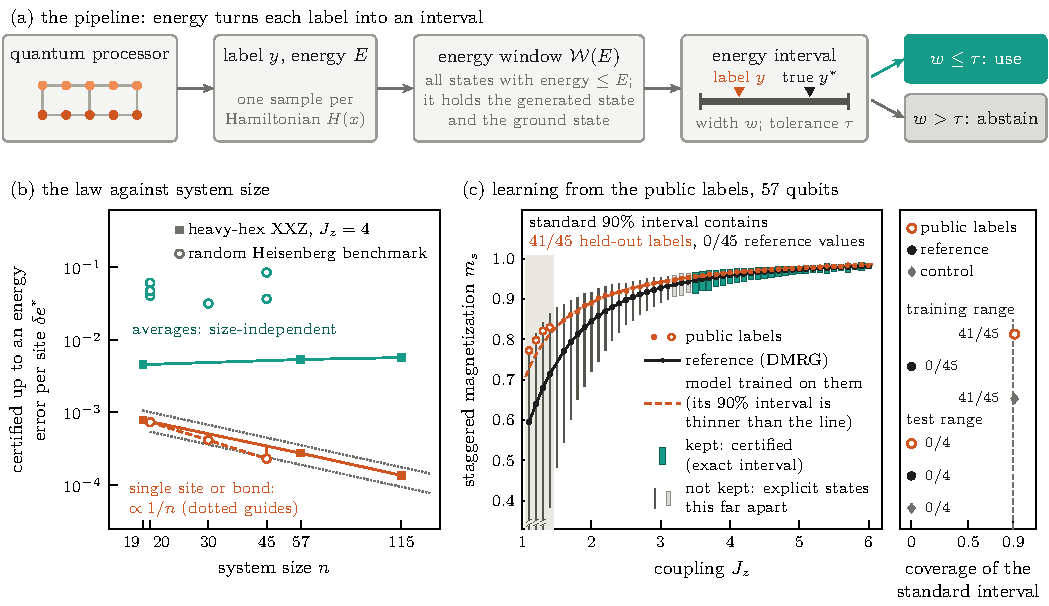
\includegraphics[width=\textwidth]{fig1_overview_rd_pgf}%
\caption{\label{fig:overview}What energy certifies, and what a learner can guarantee.
(a) A label's energy $E$ fixes an interval containing the label $y$ and its true value $y^*$; the label is used only
if the width $w$ is at most the tolerance $\tau$.
(b) Maximal energy error per site at which a label stays certified: flat for averages, falling as $1/n$ for single
sites and bonds (squares: heavy-hex XXZ at $\Jz=4$, $n=19$, $57$, $115$, from the map; circles: benchmark instances; % src: file:paper/figures/pgf_overview/export_check.txt (rows n=19,57,115, Jz=4)
bars from the inner to the outer bound, visible only at $n=45$). % src: file:phase3/full_runs/huang/RESULTS.md (n = 45)
(c) The public labels of the 57-qubit dataset. A cubic model trained on the 45 training labels (orange) and its
standard $90\%$ interval (the plain jackknife, which has no finite-sample guarantee~\cite{barber2019}; about $0.1\,\tau$ wide, thinner than the line) follow the labels, not the reference (black): % src: rdc:sizes.57.models.poly3_invJ.ood_emulated.levelM (0.9); rdc:sizes.57.models.poly3_invJ.indist_emulated.summary.widthM_tau_median (0.1033)
at the four test couplings (shaded) the model misses the reference by $2.28$--$3.73\,\tau$. Teal bars, dark rim: the exact interval of % src: file:paper/figures/pgf_overview_rd/export_check.txt (2.28-3.73 tau)
the $26$ labels kept by the energy filter (certified, from the certification map of Fig.~\ref{fig:map}). Grey bars, not kept: between the labels of two explicit % src: rdq:jstar.57_m_s.sec2.certified_exact (26)
states of the window ($19$ training labels: $16$ not certified, dark; % src: file:paper/figures/pgf_overview_rd/export_check.txt (drops 19; 16 not certified)
$3$ undecided, light; at $\Jz=1.1$--$1.3$ the bars, $13.5$--$18.8\,\tau$ wide, are cut by the axis, with a break mark). % src: file:paper/figures/pgf_overview_rd/export_check.txt (3 undecided; 13.5-18.8 tau wide)
Right (and upper left): fraction of couplings at which the standard interval contains a held-out public label (open), the reference
(black) and, for a control model trained on DMRG labels, the reference (grey): at $n=57$, $41$, $0$ and $41$ of the 45 in the % src: file:paper/figures/pgf_overview_rd/export_check.txt (41 of 45, 0 of 45, control 41 of 45)
training range (at $n=115$ the reference is inside at $11$) and none of the $4$ in the test range for all three, the control included. % src: file:paper/figures/pgf_overview_rd/export_check.txt (0 of 4, 0 of 4, control 0 of 4); rdl:summary.115.models.poly3_invJ.real.ind.truth_covered (11)
Drawn by a script written with an AI tool (Methods); panels (b) and (c) from the deposited data.}
\end{figure*}

Quantum processors have begun to supply the labels on which machine-learning models of quantum many-body ground
states are trained~\cite{cho2024,jaderberg2026}. Each label then needs a guarantee that does not come
from its generator, or a proof that a given check cannot give one. A check that scales with such data comes with
every sample: its energy. We show, label by label, what that energy guarantees about the label and what energy
accuracy a guarantee requires. One rule organizes the answer: at a fixed energy error per site, the energy keeps
certifying a label as the system grows only if moving the label costs energy linear in the system size;
single-site labels never do, and averages do under a uniform-gap hypothesis, a theorem at strong anisotropy for
the model studied here (Theorem~\ref{thm:strong}).

We apply the rule to a public dataset of $57$ and $115$ qubits~\cite{jaderberg2026,jaderberg2026data}. Its published energy and site % src: def:phase3/full_runs/real_data/DECLARATION.md (n = 57, 115)
magnetizations certify, in exact arithmetic and with no reference value, the order parameter to a tolerance
$\tau$ of $6\%$ of its ground-state value at $26$ of the $45$ training couplings at $57$ qubits and at $21$ at % src: def:phase3/full_runs/real_data/DECLARATION.md (tau = 0.06 |O_GS|); derived: 0.06 = 6 %; rdq:jstar.57_m_s.sec2 (26; 3.5); rdq:jstar.115_m_s.sec2 (21; 4.0)
$115$ ($27$ with certificates added after the analysis was declared). At those $26$ and $21$ couplings an exact % src: rdeq:jstar.115_m_s.sec2_e1 (27; 3.4); rdq:jstar.57_m_s.sec2 (26; 3.5); rdq:jstar.115_m_s.sec2 (21; 4.0)
$19$-site calculation, which uses no quantum data, already lies within $0.135\,\tau$ and $0.143\,\tau$ of the % src: rdq:filter.57_m_s.exact.classical_n19.max_over_kept (0.1344); rdq:filter.115_m_s.exact.classical_n19.max_over_kept (0.1424); derived: upper bounds ceiled, 0.1344 to 0.135 and 0.1424 to 0.143
reference value. Near the
isotropic point, where the test couplings lie and that calculation misses by more than a tolerance, explicit states
show that none of the seven labels we analysed is certified, and they bound what a guarantee there would take: an
energy error per site more than $110$ times below the published one at $57$ qubits and $79$ times at $115$ % src: rdq:accuracy_factors.57.m_s.headline_F_A (110); rdq:accuracy_factors.115.m_s.headline_F_A (79)
[Fig.~\ref{fig:landscape}(a); Secs.~\ref{sec:map} and~\ref{sec:discussion}]. The public labels are over-ordered
there, as our emulation of the first stage of the generating method had indicated (Sec.~\ref{sec:method}), and for
learning the energy intervals flag where the energy cannot vouch for a label, which validation against the
generator's own labels cannot (Sec.~\ref{sec:learn}). Figure~\ref{fig:overview} summarizes the rule and the
learning result.

These labels are magnetizations, correlation functions and order parameters at many values of a Hamiltonian
parameter, and provable learning guarantees exist when they are close to the
truth~\cite{huang2022,lewis2024,wanner2024}. The dataset studied here contains site-resolved
magnetizations, nearest- and next-nearest-neighbour correlations and loop operators of the XXZ model on heavy-hex
lattices of 57 and 115 qubits, generated by sample-based Krylov quantum diagonalization (SKQD)~\cite{yu2025skqd} on a % src: def:phase3/full_runs/map/DECLARATION.md
superconducting processor and used to train a model that is then tested outside its training
range~\cite{jaderberg2026}. Its labels, the energy of each sample and its authors' own tensor-network (DMRG) values
are public~\cite{jaderberg2026data}.

Sample-based diagonalization returns a classically stored vector in a set of sampled configurations~\cite{kanno2023,robledo2025,yu2025skqd}, so its energy is
a computable Rayleigh quotient, and energy is already used in practice to screen runs~\cite{jaderberg2026}. Other
checks exist, such as the energy variance, leakage out of the symmetry sector~\cite{chen2026} and diagnostics of the
prepared state beyond its energy~\cite{niu2026}; a comparison with a classical reference needs that reference, and in
our exact checks at $12$ sites a reported variance excludes none of the states that set the width of the energy % src: file:phase3/design/R2_constructive_half.md (n = 12)
window (Supplemental Sec.~S7). Labels, however, are not energies. A learner trained on labels with a systematic error reproduces that
error~\cite{koridon2024} (for classification, the effects of label noise are surveyed in Ref.~\cite{frenay2014}), and
validation against new data with the same error does not reveal it. The question behind the result above is therefore: \emph{which labels does a sample's energy certify, and to what precision, what
does the energy say where it certifies nothing, and what can a learner trained on such labels then guarantee about the
truth?} Distribution-free uncertainty
quantification does not answer the last part by itself: split conformal prediction calibrated on generated labels
covers new generated labels at the nominal rate~\cite{angelopoulos2021}. It covers the true ones when the label noise
only adds dispersion and can fail for a systematic error~\cite{einbinder2022}; when each label is known only up to a
set, covering every admissible truth costs intervals about as wide as the sets~\cite{cauchois2022}. The energy
supplies such a set for each label, an interval.

The ingredients of an answer are old. The energy error is quadratic in the state error~\cite{eckart1930}; expectation
values can be bounded from energy and overlap information~\cite{weinhold1968}; the extreme values of an observable over
all states below a given energy follow from Lagrange multipliers~\cite{cohen1971}. Manchanda recently assembled these
into a certification radius for variational outputs~\cite{manchanda2026}, with a two-sided $\sqrt{2\epsilon\chi}$ law
at leading order for energy errors below half a gap and an application to Krylov quantum diagonalization showing
that a well-converged energy can leave observables uncertified (Supplemental Sec.~S10). Window-constrained semidefinite and bootstrap certificates bound observables from
an energy interval~\cite{wang2024prx,wang2026scipost,vallee2026,banerjee2026}; we ask how far an energy window can
reach at any level of relaxation. The dataset paper itself notes that its
Eckart-type bound ``does not directly control local observables''~\cite{jaderberg2026}, and it reports the
unsigned errors of its site magnetizations against its own DMRG reference (its Supp.\ Fig.~11); its public record
gives $16$--$32\%$ at $57$ qubits and $14$--$30\%$ at $115$ at the four couplings % src: file:phase3/full_runs/real_data/checks/r11/fn_cite1_check_public_record_out.txt (16.74, 31.47 at n = 57; 14.77, 29.80 at n = 115); file:phase3/full_runs/real_data/checks/r11/fp_hostileB_recompute_bias_out.txt (16.7, 31.5; 14.8, 29.8); derived: ranges rounded outward
$\Jz=1.1$--$1.4$ of its out-of-distribution tests. % src: def:phase3/full_runs/real_data/DECLARATION.md (Test: 1.1-1.4)

The paper has four parts; Table~\ref{tab:status} lists what in them is proved, what depends on reference values
and what is assumed.
\begin{enumerate}
\item \emph{The rule} (Sec.~\ref{sec:rule}). Local labels lose certification beyond a size of order $\kappa/\de$
(proved; in a charge sector, for every single site at a fixed magnetization density); averages obey a
size-independent $\sqrt{\de}$ law under a uniform-gap hypothesis, proved for the dataset's model above a coupling
that is not explicit (Theorem~\ref{thm:strong}) and assumed in the dataset's range; and a criterion, which follows
from duality and the definitions, says which labels stay certifiable as $n$ grows.
\item \emph{The dataset} (Sec.~\ref{sec:dataset}). A label-by-label certification map of the public data at both
sizes, in exact arithmetic on the ``certified'' side and with explicit states on the ``not certified'' side, and
the sign and origin of the bias of the first stage of the generating method, in our emulation, in one device run
per coupling and in the public labels.
\item \emph{The bias against the energy} (Sec.~\ref{sec:predict}). For that first stage the bias lies close to one
curve per coupling in the energy error per site, found after the data were in hand and then tested under rules
fixed in writing beforehand. The curve passes its declared test on new emulated labels and fails it on the
public labels, on its second condition at $115$ qubits; corrected labels do not beat the best classical % src: def:phase3/full_runs/real_data/DECLARATION.md (n = 115)
estimates; and one processor label has an
interval proved below $\tau$, at a coupling where a classical energy does better.
\item \emph{Learning} (Sec.~\ref{sec:learn}). Energy intervals of the labels carried through a learner and its
calibration (Proposition~\ref{prop:learn}: conformal prediction with set-valued
labels~\cite{javanmardi2023,cauchois2022}, here intervals supplied by the physics, and a floor that holds for any
learner), tested on the public labels and on the public benchmark of Ref.~\cite{huang2022}: standard intervals
follow the labels, and a guarantee on predictions needs calibration on labels certified well below the tolerance.
\end{enumerate}
The certified statuses of the public labels rest on one hypothesis, that the published energy, site
magnetizations and correlations are expectation values of one state; the ``not certified'' statuses do not use it
and use the reference tolerance (Table~\ref{tab:status}). Beyond this dataset, the results give producers of
quantum-generated data the energy accuracy each label needs (Corollary~\ref{cor:law}) and a way to report what each label's energy guarantees; they give
users of such data a filter that keeps only generated labels guaranteed within $\tau$ of the truth
(Sec.~\ref{sec:learn}); and for data that cannot be checked
classically, explicit states can still prove, without the ground-state energy, that given labels are not certified
by their energy (Theorem~\ref{thm:local}(c), Proposition~\ref{prop:W}).

\begin{figure*}[t]
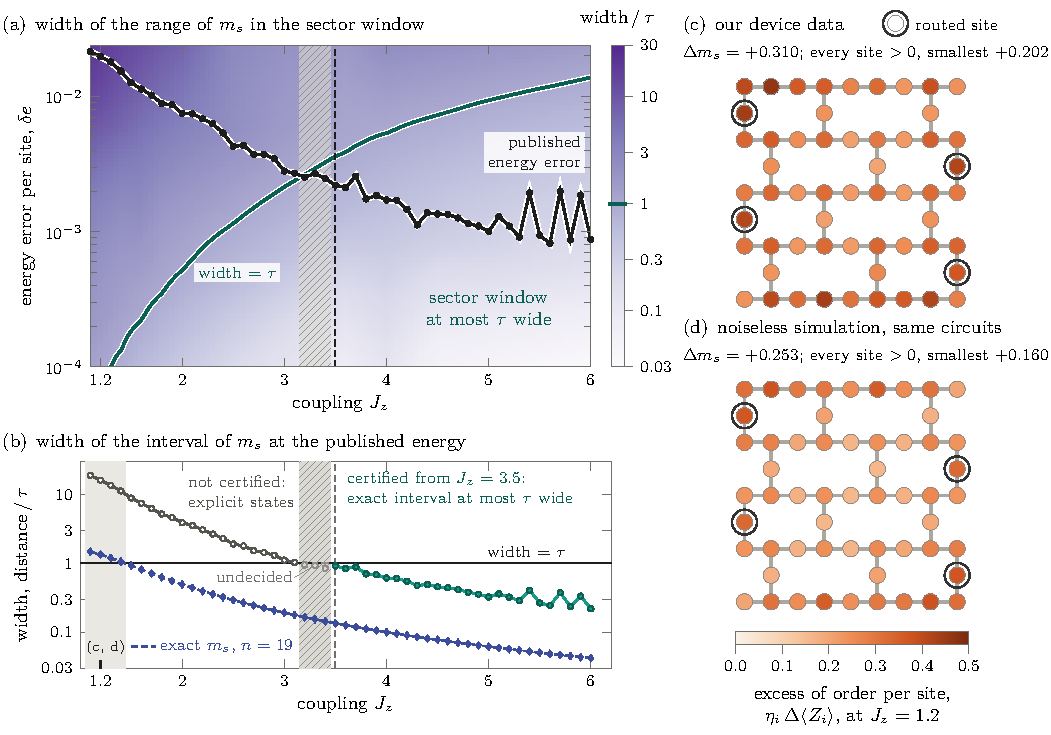
\includegraphics[width=\textwidth]{fig1_composite_rd_pgf}%
\caption{\label{fig:landscape}What a sample's energy certifies, and what the first stage of the method class does
inside the window ($n=57$). (a) The range of the staggered magnetization allowed by the energy, over the coupling $\Jz$ and the energy error per site
$\de$: the colour is the width of that range, i.e.\ the spread of $\ms$ over all sector states with an
error per site of at most $\de$ (inner side, from the stored states, as in Supplemental Fig.~S1; in units of $\tau$, log scale), a property of the model. Teal line: width $=\tau=0.06\,|m_s^{\rm GS}|$; below it the sector window is at most $\tau$ wide. % src: def:phase3/full_runs/map/DECLARATION.md (tau = 0.06|O_GS|)
Black line: the published energy error of the dataset at each of its 50 couplings (one dot per coupling, as published, its zigzag at large $\Jz$ included), the four % src: file:paper/figures/pgf_composite_rd/export_check.txt (50 couplings)
test couplings included.
(b) The width of the interval of $\ms$ at the published energy, in units of $\tau$, with the statuses of
Fig.~\ref{fig:map}. Open dark-grey circles: not certified; the distance between the labels of two explicit states of the
window, $11.1$--$18.8\,\tau$ at the test couplings (shaded). Light grey, hatched also in (a): undecided ($\Jz=3.2$--$3.4$; at $\Jz=3.4$ the % src: file:paper/figures/pgf_composite_rd/export_check.txt (11.1-18.8 tau apart at the test couplings)
bar reaches the width of the exact interval, $1.0043\,\tau$). Filled teal circles: certified; the width of the exact % src: file:paper/figures/pgf_composite_rd/export_check.txt (exact interval 1.0043 tau wide, undecided)
interval, from $0.911\,\tau$ at $\Jz=3.5$ (dashed, also in (a)) to $0.218\,\tau$ at $\Jz=6.0$. The exact interval % src: rdm:rows[n=57,Jz=3.5,label=m_s].exact.width_over_tau (0.91040); rdm:rows[n=57,Jz=6.0,label=m_s].exact.width_over_tau (0.21784); derived: both rounded up
contains the sector window of (a), so the certified range can begin only where the black line is below the teal
line.
Blue diamonds: how far the exact $\ms$ of $19$ sites, which uses no quantum data, lies from the reference of
$n=57$, in the same units: at most $0.135\,\tau$ at the $26$ certified couplings and $1.05$--$1.47\,\tau$ at the % src: file:paper/figures/pgf_composite_rd/export_check.txt (0.135, 1.05-1.47); rdp:sizes.57.n19_comparison.n_kept (26)
test couplings.
(c) Our own device data of the first stage of the sample-based Krylov method class (a superconducting heavy-hex processor, Methods;
without basis optimization; $\Jz=1.2$, one job): excess $\eta_i(\langle Z_i\rangle-\langle Z_i\rangle_{\rm DMRG})$ at % (Jz grid value)
each site ($\eta_i=+1$ on the majority colour), positive at all 57 sites ($\Delta\ms=+0.310$). The 4 ringed boundary % src: qpu:points.1.2.device.rec.dm_s (0.3098); file:phase3/full_runs/qpu/RESULTS.md (57/57)
sites were routed, at the cost of $17\%$ more two-qubit gates. % src: file:phase3/full_runs/qpu/RESULTS.md (4, +17 %)
(d) Noiseless simulation of the identical circuits, same colour scale: $\Delta\ms=+0.253$, again positive at every % src: qpu:points.1.2.control.rec.dm_s (0.2527)
site; in this one job the device noise adds $+0.057$. % src: qpu:points.1.2.D3_dm_s_device_minus_control (0.0572)
Drawn from the deposited data by a script written with an AI tool (Methods).}
\end{figure*}

\section{Setting}
\label{sec:setting}

Let $\Lambda$ be a finite graph with $n$ sites and $H=\sum_X h_X$ a finite-range Hamiltonian. The rule of
Sec.~\ref{sec:rule} is stated for states of a charge sector with projector $\Pi$ (here a fixed $S^z$, the sector of
the ground state). For a threshold $E$, the \emph{window}
\begin{equation}
\W(E)=\{\sigma\succeq0,\ \Tr\sigma=1,\ \Pi\sigma\Pi=\sigma,\ \Tr H\sigma\le E\} % (formula)
\label{eq:window}
\end{equation}
contains every state, pure or mixed, that the energy $E$ cannot exclude, including the ground state. For a label $O$
the \emph{information limit} is the interval $I_O(E)=\{\Tr O\sigma:\sigma\in\W(E)\}=[o^-(E),o^+(E)]$, of width
$w_O(E)$; at a label's own energy we call it its \emph{energy interval}. We write $E_0$ for the sector ground energy, $\epsilon=E-E_0$, $\de=\epsilon/n$, and $o_\GS^\pm$ for the maximum
and minimum of $\langle O\rangle$ over the sector ground states ($o_\GS$ when the ground state is unique). Any certificate whose
soundness rests only on membership in $\W(E)$---window semidefinite or bootstrap
relaxations~\cite{wang2024prx,wang2026scipost,vallee2026,banerjee2026}, and Eckart or radius
bounds~\cite{eckart1930,manchanda2026}---returns an interval of width at least $w_O(E)$, provided it
uses only the energy constraint and positivity; bounds that also use the overlap or the variance of the label in the
generated state, such as Weinhold's~\cite{weinhold1968}, and certificates that add eigenstate or ground-state optimality
conditions~\cite{araujo2023,fawzi2024,scheer2025} are not covered. A label is \emph{certified} at tolerance $\tau:=0.06\,|o_\GS|$ when % src: def:phase3/full_runs/map/DECLARATION.md (tau = 0.06|O_GS|)
$w_O\le\tau$, and $\des(O)$ denotes the greatest $\de$ at which this holds. Since a generated state of the sector and
the ground state both lie in the window, a certified label is within $\tau$ of the ground-state value, i.e.\ within $6\%$ of % src: def:phase3/full_runs/map/DECLARATION.md (tau = 0.06|O_GS|); derived: tau/|o_GS| = 6 %, tau/2 = 3 %
$|o_\GS|$; only the midpoint of the window is guaranteed to within $\tau/2$. At the dataset, $o_\GS$ in $\tau$ is a
DMRG reference value (Methods).

\emph{Energy and mean magnetization.} The public data of Sec.~\ref{sec:dataset} call for a second window. With
$M_z=\sum_iZ_i$,
\begin{equation}
\W(E,M)=\{\sigma\succeq0,\Tr\sigma=1,\Tr H\sigma\le E,\Tr M_z\sigma=M\} % (formula)
\label{eq:windowM}
\end{equation}
has no sector projector: it fixes only the mean of $M_z$. We write $M_0$ for the value of $M_z$ in the N\'eel
sector, $E_{\rm pub}$ for a published energy, $M_{\rm pub}=\sum_i\langle Z_i\rangle$ for the sum of the published site
magnetizations, and $q=(M_0-M_{\rm pub})/2$. The
sector window is contained in $\W(E,M_0)$, and on the public data \emph{certified} means that the interval proved
for all of $\W(E_{\rm pub},M_{\rm pub})\cup\W(E_{\rm pub},M_0)$ is at most $\tau$ wide (Sec.~\ref{sec:map}).

The sector constraint $\Pi\sigma\Pi=\sigma$ in Eq.~\eqref{eq:window} is an assumption about a generated state, and
some constraint on the magnetization is needed: with none at all, an order parameter whose orientation the sector
fixes is not certified at any accuracy, because the states of opposite total magnetization are exactly degenerate
and the window of the staggered magnetization contains both orientations at any $\de>0$. With a fixed mean,
in $\W(E_0+n\de,M)$, the reversed sector has weight at most $(M_0-M)/(2M_0)+\de/(2m_0B_+)$, with
$m_0=M_0/n$ and $B_+$ the least energy per unit of magnetization above the sector: a part that a deficit of the
mean allows at no energy cost, $q/M_0$ at the published mean, and a part proportional to the error per site and
independent of $n$ (Supplemental Sec.~S1, with its condition, which we verified at $12$ and $19$ sites only). The bound is % src: file:phase3/full_runs/real_data/checks/r11/ft_mean_window_comb_and_n19_out.txt (comb: n=12; n = 19 patch: interval of fields (B_-, B_+))
attained in an exact $12$-site example (Supplemental Sec.~S2); no status of the dataset uses it. % src: file:phase3/full_runs/real_data/checks/r11/ft_mean_window_comb_and_n19_out.txt (comb: n=12; greatest weight of the reversed sector = bound)
The statements of Sec.~\ref{sec:rule} are for the
sector window; the statuses of the public data use $\W(E,M)$ and do not assume in-sector states.

\begin{lemma}[Lagrange duality~\cite{cohen1971}]
\label{lem:dual}
For $\epsilon>0$, $o^+(E_0+\epsilon)=\inf_{\lambda>0}[E_0+\epsilon-E_0(H-\lambda O)]/\lambda$, with all ground
energies taken in the sector. When the infimum is attained, the extremal state is a ground state of $H-\lambda^*O$,
or a mixture of two across a level crossing; it is not attained when the label saturates inside the window
($\lambda\to\infty$). For any $L(\lambda)\le E_0(H-\lambda O)$ and every $\sigma\in\W(E)$,
$\Tr O\sigma\le[E-L(\lambda)]/\lambda$. With two constraints: for any real $\mu$ and any $L(\lambda,\mu)$ not above
the lowest eigenvalue of $H-\lambda O+\mu M_z$ on the full space, every $\sigma\in\W(E,M)$ has
$\Tr O\sigma\le[E+\mu M-L(\lambda,\mu)]/\lambda$.
\end{lemma}

\begin{lemma}[Pure witnesses suffice]
\label{lem:pure}
The joint numerical range of $(\Pi H\Pi,\Pi O\Pi)$ over pure states is convex (Toeplitz--Hausdorff~\cite{toeplitz1918,hausdorff1919}).
Hence every width below is attained by pure states, in general with complex coefficients; a mixture of two
matrix-product states with bond dimensions $\chi_a,\chi_b$ is replaced by a pure state of bond dimension at most
$\chi_a+\chi_b$ in their span.
\end{lemma}

\section{The rule}
\label{sec:rule}

Lemma~\ref{lem:dual} and the leading-order law are known (Sec.~\ref{sec:discussion}), and
Theorems~\ref{thm:local}--\ref{thm:cost} follow from Lemma~\ref{lem:dual} and standard perturbation theory; what this
section adds is uniformity in the system size, the resulting classification of which labels stay certifiable as $n$
grows, its proof for the dataset's model at strong anisotropy (Theorem~\ref{thm:strong}), and its use on a dataset
(Sec.~\ref{sec:dataset}).
Proofs are in the Supplemental Material~\cite{SM} (Secs.~S1 and~S16); each statement of % (structural: section numbers)
Theorems~\ref{thm:local}--\ref{thm:cost} and their corollaries was attacked numerically on exact
diagonalizations of lattices of up to $12$ sites (Ising and XXZ % src: file:phase3/design/R3_generality.md (n <= 12)
models, local and averaged labels), about $300$ checks in all with no violation (Sec.~S2; tightness: Sec.~S12). % src: file:phase3/design/R3_generality.md (about 300)

\emph{Local labels.} Let $O$ be supported on a region $A$ and let
$\kappa_A=\sum_{X\cap A\neq\emptyset}[\lambda_{\max}(h_X)-\lambda_{\min}(h_X)]$ be the energy spread of the terms that
touch $A$.

\begin{theorem}[Local labels]
\label{thm:local}
(a) Without a sector constraint, for every $\epsilon\ge0$ the upper extent satisfies
$o^+(E_0+\epsilon)-o_\GS^+\ge\min(1,\epsilon/\kappa_A)\,(o_{\max}-o_\GS^+)$, and likewise below. Hence at fixed error
per site the information limit is the full spectral range of $O$ for all $n\ge N^*_O(\de):=\kappa_A/\de$.
(b) In a sector of a U(1) charge that is a sum of on-site charges, for $O$ commuting with the charge of a block
$B\supseteq A$, the same holds with a
covariant measure-and-prepare channel on $B$: the extent is at least $\min(1,\epsilon/\kappa_B)(c_B^+-o_\GS)$, with
$c_B^+=\sum_q p_q\lambda_{\max}(O|_q)$, $O|_q$ the restriction of $O$ to block charge $q$ and $p_q$ the ground-state
distribution of the block charge; for $O=Z_i$, $c_B^+=1-2P(\text{block fully down})$.
(c) The construction is free of $E_0$: if $\phi$ is any explicit sector state with $\langle H\rangle_\phi\le E$,
every energy-only certificate at $E$ has width at least
$\min\{1,(E-\langle H\rangle_\phi)/\kappa_B\}\,[c_B^+(\phi)-c_B^-(\phi)]$.
(d) Without a sector constraint, with $\kappa_1=\max_i\kappa_{\{i\}}$ the maximal single-site spread, the window of a
label averaged over $b$ sites is its full range once $n\de\ge b\kappa_1$, that is, for every $b\le b^*=n\de/\kappa_1$,
and the label is then not certified at any tolerance below its range; in a sector the construction reaches
$c_B^\pm$ as in (b), a lower bound on the extent.
\end{theorem}

No non-commutation hypothesis is needed and the gap does not enter. The reset bound is attained for non-interacting
spins and loose otherwise by a model-dependent factor (about six for a single site of a transverse-field Ising % src: file:paper/reviews/R10_2026-11-12/scratch/math-thm1/t3_looseness_output.txt (N*/that = 6.12); derived: rounded
chain at $h=1.5$), and certification at tolerance $\tau$ is lost far before $N^*$ % src: file:paper/data/crosschecks/check2_output.txt (h=1.5)
(Corollary~\ref{cor:law}; Supplemental Secs.~S1 and~S12). % (structural: section numbers)

\emph{Intensive averages.} Let $\bar O=\frac1n\sum_io_i$ with local $\|o_i\|\le1$, $f_n(\mu)=E_0(H-\mu n\bar O)/n$, and
$\alpha_n(\mu)=f_n(0)-\mu\bar o_\GS-f_n(\mu)\ge0$, a convex function. Let $u_n(\de)=o^+(E_0+n\de)-\bar o_\GS$.

\begin{theorem}[Intensive averages]
\label{thm:avg}
(a) $u_n(\de)=\inf_{\mu>0}[\alpha_n(\mu)+\de]/\mu$: only energy densities enter, and the extremal states are ground
states of $H-\mu n\bar O$, a uniform conjugate field.
(b) With $\chi_\pm(\mu_1)=\sup/\inf_{0<\mu\le\mu_1}2\alpha_n(\mu)/\mu^2$,
\begin{equation}
\min\{\sqrt{2\chi_-\de},\ \chi_-\mu_1/2\}\ \le\ u_n(\de)\ \le\ \sqrt{2\chi_+\de} % (formula)
\label{eq:sandwich}
\end{equation}
for all $\de\le\chi_+\mu_1^2/2$, and $u_n(\de)\le\sqrt{2\chi\de}$ for all $\de$ if and only if $\alpha_n(\mu)\le\chi\mu^2/2$
for all $\mu$.
(c) If, for every $\mu\in[0,\mu_1]$, $H-\mu n\bar O$ has a unique sector ground state with gap at least $\Delta_*$ and
connected correlations obeying $\max_i\sum_j|\langle o_io_j\rangle_c|\le C_1$ (so $\Delta_*$ and $C_1$ are the
infimum and supremum along the deformed family), then $\chi_+(\mu_1)\le2C_1/\Delta_*$ uniformly in $n$; when the
$o_i$ commute with the charge and $H$ has finite-range terms of bounded norm on graphs of bounded degree and
polynomial growth, such a $C_1$ exists and depends only on $\Delta_*$, $\mu_1$ and these local data (Supplemental
Sec.~S1), so the gap is the only hypothesis. No condition
on $\epsilon/\Delta$ is required. The lower extent obeys the same statements with $\bar O\to-\bar O$.
(d) If the sector ground state is not an eigenvector of $\bar O$, $u_n(\de)=\sqrt{2\chi_n(0)\de}\,[1+O(\sqrt{\de})]$; if it
is, $u_n(\de)\le\de/\mu_c$ with $\mu_c$ the field at which the ground state changes.
\end{theorem}

Uniformity in $n$ therefore rests on (c): it holds wherever the deformed family stays gapped and clustered, and it
can fail on the side that opposes a pinned order, where the family can cross to a reversed-domain state at a field
that decreases with $n$ (an exact example, and the extensive width of a pinned comb above the gap: Supplemental
Sec.~S12). For the dataset's model (c) is a theorem at strong anisotropy (Theorem~\ref{thm:strong} below); in the
dataset's range the uniform sector gap along the deformed family remains a hypothesis at $n=57$ and $115$. For $\ms$
on the heavy-hex patches the classical part of the family cannot cross below $|\mu|=\Jz/32$ at any size, and the % (formula)
bound on $C_1$ obtained from the gap is far from the computed values (Supplemental Sec.~S1).
Without a gap the law changes form: with Goldstone modes in two dimensions $u\propto\de^{1/3}$ at leading % (formula)
order~\cite{hofmann2020}, a window that published iPEPS states~\cite{hasik2021} neither contradict nor show to be
tight (Supplemental Sec.~S15).

\emph{The general criterion.} Define the cost of moving a label by $c$ inside the sector,
$E_n^*(c)=\min\{\Tr H\sigma-E_0:\Tr O\sigma\ge o_\GS+c\}$, and $E_n^*(-c)$ likewise with $\Tr O\sigma\le o_\GS-c$.

\begin{theorem}[Cost of moving a label]
\label{thm:cost}
(a) $o^+(E_0+\epsilon)-o_\GS\ge c$ if and only if $\epsilon\ge E^*_n(c)$, and $E^*_n$ is the convex conjugate of
$\alpha$.
(b) Energy-only certification of $O$ to precision $c$ at error per site $\de$ therefore holds at size $n$ if and only
if $E^*_n(c)>n\de$; $O$ is certifiable at some fixed $\de>0$ for all sufficiently large $n$ if and only if
$\liminf_nE^*_n(c)/n>0$.
(c) Local labels and averages over $o(n)$ sites have $E^*_n=o(n)$ and are uncertifiable at large $n$ (in a sector,
when a block of bounded size has reset values that differ from $o_\GS$ by a fixed amount, as every single site
does at a fixed magnetization density). Any average
whose deformed family satisfies Theorem~\ref{thm:avg}(c) on both sides, with $\Delta_*$, $C_1$ and $\mu_1$
independent of $n$, has $E^*_n(\pm c)\ge nc^2/(2\bar\chi)$ for $c\le\bar\chi\mu_1$, where $\bar\chi=2C_1/\Delta_*$,
and is certifiable.
\end{theorem}

Part (a) is the Legendre duality between the ground energy in a conjugate field and the constrained minimum energy,
the structure of Lieb's formulation of density-functional theory~\cite{lieb1983} with $O$ in place of the density;
the content is in (c), which says which labels have a linear cost.
A sector-pinned order parameter is covered by (c) only if Theorem~\ref{thm:avg}(c) holds also on the side that
opposes the order, which can fail (see after Theorem~\ref{thm:avg}). The heavy-hex sectors of the dataset fix the total
magnetization (Methods), which pins the orientation of the staggered order.
Two classes with sublinear cost are proved in Supplemental Sec.~S1: an order parameter that no sector and no
boundary pins, after Horsch and von der Linden~\cite{horsch1988,koma1994}, and an order fixed only by a boundary
or by a sector of bounded net charge, which is reversed, in any region with a symmetry that exchanges its two
sublattices, at the cost of the region's boundary terms. On the heavy-hex patches this construction gives no
sublinear cost, since every region with such a symmetry has at least $|R|/6$ crossing bonds. The critical class % (formula)
remains heuristic (Supplemental Sec.~S12).

\begin{theorem}[Uniform gap and linear cost at strong anisotropy]
\label{thm:strong}
Let $H=\frac14\sum_{\langle ij\rangle}(X_iX_j+Y_iY_j+\Jz Z_iZ_j)$ on the heavy-hex patch of odd distance $d\ge3$
[$n=(5d^2-2d-1)/2$ sites; $d=5$ and $7$ are the dataset's graphs], in the sector of its N\'eel configuration, let % (structural: distances of the dataset's graphs)
$\bar O$ be $\ms$, $\Czz$ or $\Ctwo$ (Sec.~\ref{sec:dataset}), and let $0<c_0<3/104$, $1/56$ or $3/416$, % (formula)
respectively. There are constants $J_c<\infty$, $\delta_0>0$ and $\bar C_1<\infty$, depending only on the label and
on $c_0$, such that for every $d$, every $\Jz\ge J_c$ and every $|\mu|\le\mu_1=c_0\Jz$ the sector ground state of
$H-\mu n\bar O$ is unique, with sector gap at least $\delta_0\Jz$, exponentially decaying connected correlations and
$\mathrm{Var}(n\bar O)\le n\bar C_1$, and it is the non-degenerate ground state of $H-\mu n\bar O-\frac38\Jz M_z$ on
the full space. Hence $\alpha_n(\mu)\le\bar\chi\mu^2/2$ with $\bar\chi=2\bar C_1/(\delta_0\Jz)$, and
$E^*_n(\pm c)\ge nc^2/(2\bar\chi)$ for $0\le c\le\bar\chi\mu_1$: each of the three labels is certifiable at a
fixed error per site at every size. The same holds on periodic heavy-hex lattices, and the ground states converge
to a gapped pure state of the infinite lattice.
\end{theorem}

The proof (Supplemental Sec.~S16) combines a site-by-site lower bound on the classical energy of the patches, open
boundary included, verified in exact arithmetic, with the stability theorem of Nachtergaele, Sims and Young for
frustration-free models~\cite{nsy2022}, whose hypotheses we verify for the open patches, and with the clustering
theorem of Ref.~\cite{nachtergaele2006}. It has two limits. The constants are not usable: $J_c$ is not explicit,
and for every window and every $\delta_0$ that the proof can give the formula for $\bar C_1$ exceeds $10^{26}$, where exact % src: file:phase3/full_runs/real_data/checks/r11/ft_theorem4_constant_out.txt (C1bar=1.5308e+26 in the limit delta_0 -> 3/52, c_0 -> 0); derived: rounded down
diagonalization at $n=19$, $\Jz=6$ gives a correlation sum of $0.11$; the theorem states that a size-independent % src: file:paper/reviews/R10_2026-11-12/scratch/rw-V/v_item4_ed19_out.txt (0.1134); derived: rounded
error per site exists, not its value. And the dataset's range $\Jz=1.6$--$6.0$ is not covered: there the uniform
gap remains an assumption (Table~\ref{tab:status}), consistent with exact diagonalization at $n=19$ and with the
computed intensivity at $n=57$ and $115$. The full-space statement cannot reach the lower part of that range: at
$n=19$ it fails at $\Jz=1.6$ for $\mu=0$ and, for $\ms$ with the opposing tilt $\mu=-\Jz/40$, at every computed % src: file:paper/reviews/R10_2026-11-12/scratch/rw-V/v_item4_ed19_out.txt (no tilt           -0.0321; m_s, -1/40)
coupling up to $\Jz=4.0$ (it holds at $4.5$), so $J_c$ exceeds $1.6$ and $4.0$ for windows that contain these % src: file:paper/reviews/R10_2026-11-12/scratch/rw-V/v_item4_ed19_out.txt (-0.0670  +0.0163; 1.6, 4.0, 4.5)
tilts, while the sector gap there stays at least $0.64$. % src: file:paper/reviews/R10_2026-11-12/scratch/rw-V/v_item4_ed19_out.txt (0.6403); derived: rounded down
In $\W(E_0+\epsilon,M)$ the same bound holds with $\epsilon$ replaced by $\epsilon+\frac38\Jz(M_0-M)$ % (formula)
(Supplemental Sec.~S16). % (structural: section number)

\begin{corollary}[Accuracy law]
\label{cor:law}
The information limit reaches a shift of $\pm c$ exactly when the error per site is at least
$\des_n(\pm c)=E^*_n(\pm c)/n$, with no approximation in $\epsilon$; below it the label is certified to precision $c$
on that side. To leading order, for an interval of width $\tau$ ($c=\tau/2$ on each side),
\begin{equation}
\des=\frac{\tau^2}{8\chi}, % (formula)
\label{eq:law}
\end{equation}
with $\chi$ the per-site susceptibility of $\bar O$ to its conjugate field; for a local label
$\des=\tau^2/(8n\chi_i)$ until the full-range ceiling of Theorem~\ref{thm:local}.
\end{corollary}

At leading order Eq.~\eqref{eq:law} is the accuracy target of Ref.~\cite{manchanda2026} written per site. With
$\chi=\chi(0)$ it is an estimate, not a bound: on the side opposing a pinned order the relevant constant
$\sup_\mu2\alpha/\mu^2$ is reached at a finite field, and in exact checks on four bipartite trees it is $1.8$--$4.1$ % src: file:phase3/full_runs/learning_ibm/crosschecks/thm_attack_output.txt (chi_glob 2.15766/1.01041, 4.32830/2.45903, 1.67264/0.40529); derived: ratios 1.76-4.13
times $\chi(0)$, so Eq.~\eqref{eq:law} can overstate $\des$ by that factor.

\emph{Bounds without a ground-state energy.} The windows of a dataset are set by its reported energies $E_{\rm dev}$.

\begin{proposition}[Witness bound]
\label{prop:W}
Let $\phi_\pm$ be explicit sector states (or mixtures) with $\langle H\rangle_{\phi_\pm}\le E$ and
$D=\langle O\rangle_{\phi_+}-\langle O\rangle_{\phi_-}$. Every energy-only certificate at any $E'\ge E$ has width at
least $D$, and for every real $o$---in particular the unknown $\langle O\rangle_\GS$---one of the two states has
$|\langle O\rangle_{\phi_\pm}-o|\ge D/2$. The same holds for $\W(E,M)$ with explicit states of mean magnetization
$M$.
\end{proposition}

It needs no knowledge of $E_0$, only explicit states of energy at most the
reported $E_{\rm dev}$. (That a generated sector state itself lies in $\W(E_{\rm dev})$ holds automatically when
$E_{\rm dev}$ is its Rayleigh quotient.) Lemma~\ref{lem:dual} supplies the other side from lower bounds on tilted
ground energies, which are as reliable as the references unless proved exactly (Methods; Sec.~\ref{sec:map}).

\emph{Shifted labels.} The extremal states of Theorem~\ref{thm:avg} are ground states of $H(x)-\mu(x)n\bar O$, a
local Hamiltonian family of the same locality as the dataset's family $H(x)$.

\begin{corollary}[Single shifted labels are learnable and invisible]
\label{cor:learn}
(a) Under the gap and clustering conditions of Theorem~\ref{thm:avg}(c), and if the optimal field $\mu(x)$ at $\de(x)$ varies smoothly
with $x$, the label map of an average shifted by up to $u_n(\de(x))$ is the ground-state label map of a gapped local
family, inside the class covered by ground-state learning guarantees~\cite{huang2022,lewis2024,wanner2024}.
(b) Labels that all come from one state of the window per input, with that state's energy, are what an honest
generator at that energy could return. No procedure that uses only these labels and their energies, in particular no
validation against new labels whose quality is guaranteed only by their energy, can tell them from labels with a
smaller error.
\end{corollary}

Part (b) holds per label and for shifts realized by one state per input. It fails for label sets taken from
different states at the same input: when a combination of the labels fixes the energy, the joint set implies an
energy that the reported one contradicts, and a one-line consistency check exposes it (Sec.~\ref{sec:bench}).

\section{A 57- and 115-qubit dataset}
\label{sec:dataset}

\subsection{The certification map}
\label{sec:map}

\emph{The dataset and its public record.} The dataset of Ref.~\cite{jaderberg2026} uses
$H=\frac14\sum_{\langle ij\rangle}(X_iX_j+Y_iY_j+\Jz Z_iZ_j)$ on heavy-hex graphs with $n=57$ and $115$ sites, with
training points $\Jz=1.6,1.7,\dots,6.0$ ($45$ points) and an out-of-distribution (OOD) test at $\Jz=1.1$--$1.4$. % src: file:phase3/STEP0_witness_prior_art_feasibility.md (45 points)
Its labels are $\langle Z_i\rangle$, nearest- and next-nearest-neighbour $\langle Z_iZ_j\rangle$ and 12-site loops; the % src: file:phase3/STEP0_witness_prior_art_feasibility.md (12-site loops)
staggered magnetization $\ms=\frac1n\sum_i\eta_i\langle Z_i\rangle$ is derived from the site labels. We analyse $\ms$,
the edge average $\Czz$, the next-nearest-neighbour average $\Ctwo$, and four local labels (a bulk site, a boundary
site, one edge correlation, one loop). The public repository of the dataset~\cite{jaderberg2026data} holds at $50$ couplings $\Jz=1.1,1.2,\dots,6.0$ and both sizes the % src: def:phase3/full_runs/real_data/DECLARATION.md (k = 11..60: 50 couplings)
energy of each sample, its labels, and the authors' own DMRG values. These agree with our references (to
$3.01\times10^{-5}$ in the ground energy); the dataset paper reports label errors against them, and so do we. % src: rdg:G4_115.max_abs_dE0 (3.010e-5, the larger of the two sizes)
The published states are not in the N\'eel sector: the last step of the generating method rotates pairs of qubits and does not conserve $M_z$, and the published site magnetizations
sum to $M_{\rm pub}<M_0$ at all $100$ points (deficit $0.0003$--$0.2342$ at $n=57$, $0.0026$--$0.4353$ at $n=115$). % src: file:phase3/full_runs/real_data/RESULTS.md (negative at 50 of 50 couplings at both sizes; -0.2342 to -0.0003; -0.4353 to -0.0026); rdm:rows[n=57,Jz=1.1,label=m_s].M_real_minus_M0 (-0.234198); derived: 2 x 50 = 100, ends rounded outward
Every status below therefore refers to the window of energy and mean magnetization $\W(E,M)$ of
Sec.~\ref{sec:setting}, not to the sector window. Every certified status rests on one hypothesis, H: the published
energy $E_{\rm pub}$ and the published site magnetizations and nearest-neighbour correlations are expectation values
of one and the same state. A necessary condition, one inequality per point whose bound is built edge by edge, holds
at all $100$ points; H cannot be proved from the files. Figures~\ref{fig:landscape} % src: file:phase3/full_runs/real_data/RESULTS.md (100 points)
and~\ref{fig:map} show the map; the record, the checks and every interval are in Supplemental Sec.~S17.

\emph{Certified.} A label is \emph{certified} when the interval $I$ proved for every state of
$\W(E_{\rm pub},M_{\rm pub})\cup\W(E_{\rm pub},M_0)$ is at most $\tau$ wide. Under H it contains the published label; it
also contains the value of every sector state of energy at most $E_{\rm pub}$, hence of the sector ground state
(explicit sector states, our DMRG states, have lower energy). $I$ follows, in rational arithmetic and with no
reference computation, from the published energy and magnetization and from $140$ lower bounds on the tilted % src: rdq:certificates.n_used (140)
Hamiltonian, valid on the full space and each proved by exact integer arithmetic (Methods). With
$\tau=0.06|o_\GS|$, $\ms$ is certified at $26$ of the $45$ training couplings at $n=57$ ($\Jz=3.5$--$6.0$) and at $21$ % src: def:phase3/full_runs/real_data/DECLARATION.md (tau = 0.06 |O_GS|); rdq:jstar.57_m_s.sec2 (26; 3.5); rdq:jstar.115_m_s.sec2 (21; 4.0)
at $n=115$ ($\Jz=4.0$--$6.0$), and $\Czz$ at $27$ ($\Jz=3.4$--$6.0$) and $21$ ($\Jz=4.0$--$6.0$). The counts are the % src: rdq:jstar.57_Czz_bar.sec2 (27; 3.4); rdq:jstar.115_Czz_bar.sec2 (21; 4.0)
same with a tolerance that uses no reference, $6\%$ of the lower end of $|O|$ over $I$: the certified statuses need % src: def:phase3/full_runs/real_data/DECLARATION.md (tau_rf = 0.06 min |O| over I); rdq:jstar.57_m_s.sec2_rf.certified_exact (26)
no reference value. One row inside the range of the certificates is not within the tolerance and stays undecided: $\ms$ at $n=57$,
$\Jz=3.4$, whose interval is $1.0043\,\tau$ wide ($0.9860\,\tau$ for sector states alone), while its two explicit % src: file:phase3/full_runs/real_data/RESULTS.md (1.0043; 0.9860 at M_0 alone); rdm:rows[n=57,Jz=3.4,label=m_s].exact.width_over_tau (1.00424)
states are $0.844\,\tau$ apart. At $n=115$ certificates % src: file:phase3/full_runs/real_data/checks/r11/ft_hypothesis_H_and_explicit_widths_out.txt (n=57 Jz=3.4 explicit 0.8442); derived: rounded down
existed only at $\Jz=4.0$ and $6.0$ when the analysis was declared; an extension declared with it and computed
afterwards (Methods) raises $\ms$ there from $21$ to $27$ couplings % src: rdeq:jstar.115_m_s.sec2_e1 (27; 3.4); rdeq:jstar.115_m_s.sec2 (21)
($\Jz=3.4$--$6.0$) and $\Czz$ to $25$ ($\Jz=3.6$--$6.0$). At $n=57$ it gives intervals at $\Jz=3.3$ and $3.2$ that are % src: rdeq:jstar.115_Czz_bar.sec2_e1 (25; 3.6)
$1.12$ and $1.16\,\tau$ wide and certifies neither row. % src: rdew:rows[n=57,Jz=3.3,label=m_s].exact_e1.width_over_tau (1.11441); rdew:rows[n=57,Jz=3.2,label=m_s].exact_e1.width_over_tau (1.15321); derived: widths rounded up

\emph{Not certified.} Here explicit states decide: mixtures of stored DMRG states that have the published mean
magnetization and at most the published energy (Methods). Two of them have labels at least $\tau$ apart for $\ms$
and $\Czz$ at $\Jz=1.1$--$3.1$ ($n=57$) and $\Jz=1.1$--$3.0$ ($n=115$), and for all seven labels at $\Jz=1.1$--$1.5$, % src: file:phase3/full_runs/real_data/RESULTS.md (m_s and Czz_bar: Jz = 1.1-3.1 and 1.1-3.0; all seven labels at 1.1-1.5)
which contains the four test couplings. At $n=57$, $\Jz=1.1$ they have $\ms=0.107$ and $0.779$, $18.8\,\tau$ apart, % src: rdm:rows[n=57,Jz=1.1,label=m_s].explicit.witness_interval (0.10652, 0.77888); rdm:rows[n=57,Jz=1.1,label=m_s].explicit.width_over_tau (18.825)
around the reference value $0.595$ (public label: $0.772$). To certify $\ms$ at the test couplings, the published % src: rdm:rows[n=57,Jz=1.1,label=m_s].O_GS (0.59525); rdm:rows[n=57,Jz=1.1,label=m_s].label_real (0.77220)
energy error per site would have to be more than $110$ times smaller at $n=57$ % src: rdq:accuracy_factors.57.m_s.headline_F_A (110)
and more than $79$ times at $n=115$; for $\Czz$, more than $57$ and $49$ times (lower bounds; Methods). No % src: rdq:accuracy_factors.115.m_s.headline_F_A (79); rdq:accuracy_factors.57.Czz_bar.headline_F_A (57); rdq:accuracy_factors.115.Czz_bar.headline_F_A (49)
certificate was computed for $\Ctwo$ or the local labels, so none of their rows can be certified under this rule; at
$n=57$ the local labels are not certified at $42$ to $45$ of the $45$ training couplings. % src: rdq:jstar.57_Z_bulk.sec2.not_certified (42); rdq:jstar.57_Z_loop.sec2.not_certified (45)

\emph{Undecided.} Neither side decides $\ms$ at $\Jz=3.2$--$3.4$ ($n=57$) and $\Jz=3.1$--$3.9$ ($n=115$; $\Jz=3.1$--$3.3$ % src: file:phase3/full_runs/real_data/RESULTS.md (m_s: Jz = 3.2-3.4 and 3.1-3.9)
with the added certificates), nor a number of rows of the other labels (Supplemental Sec.~S3). For sector
states alone at the published energy, the bulk-site and single-edge labels at $n=57$, $\Jz=6.0$ are within $\tau$
($0.9770$ and $0.9737\,\tau$, DMRG-referenced): a claim fixed in advance for the figures-based map, that no local % src: file:phase3/full_runs/real_data/RESULTS.md (0.9770 and 0.9737 tau); rdm:rows[n=57,Jz=6.0,label=Z_bulk].like.w_out_over_tau (0.97698)
label is certified at any computed point, fails in that form; in the window of energy and mean magnetization these
two rows are undecided, since no certificate was computed for a local label.

\emph{Where the public labels sit.} All $100$ public $\ms$ labels lie on the over-ordered side of the reference % src: file:phase3/full_runs/real_data/RESULTS.md (positive at all 100)
[Sec.~\ref{sec:method}; Fig.~\ref{fig:map}(c, d)], and
every certified label lies within $0.175\,\tau$ ($n=57$) and $0.064\,\tau$ ($n=115$) of it. % src: rdq:filter.57_m_s.exact.miss_kept.max (0.17453); rdq:filter.115_m_s.exact.miss_kept.max (0.06390)

\emph{Agreement with the figures-based map.} A map that we had built earlier from energies digitized from the
dataset paper's figures agrees with this one row by row (Supplemental Sec.~S3); the agreement had been seen before
the analysis of the public data was declared and is a consistency check, not a blind prediction.

\emph{What the theorems add here.} The statements of Sec.~\ref{sec:rule} concern the model, in the sector, and the
numbers of this paragraph are DMRG-referenced thresholds of the model, not properties of the public labels. Every
certified row lies where the two-sided bound of Ref.~\cite{manchanda2026} holds, at errors up to half a gap
defined there (published error at most $0.05$ of the % src: map:row(115,4.0,m_s).eps_over_gap_in; derived: maximum 0.0427, at n = 115 and Jz = 4.0, of eps_pub times eps_over_gap_in over eps_dig, taken over the certified rows of the stored map
in-sector gap where the gap is stored, $0.07$ with the added certificates); what Sec.~\ref{sec:rule} adds is the % src: map:row(115,3.6,m_s).eps_over_gap_in; derived: maximum 0.0655, at n = 115 and Jz = 3.6, of the same ratio over the rows certified with the added certificates, rounded up
size dependence: which statuses
survive from $n=57$ to $115$, and why no local label stays certifiable at larger $n$. On the averaged rows with
$\Jz\ge2.0$, the set fixed in advance, the thresholds of the averages do not drift,
$\des(115)/\des(57)=1.00$--$1.17$, while the bulk site follows $0.496$, against $57/115=0.4957$ for a threshold % src: map:claims.C-E.rows (1.0007-1.1720; 0.4958); derived: 57/115 = 0.49565
that falls as $1/n$ [Corollary~\ref{cor:law}; Theorem~\ref{thm:local} bounds it from above; Fig.~\ref{fig:overview}(b)].
The accuracy law of Eq.~\eqref{eq:law} against these thresholds, which left its declared band at six rows, is in Supplemental Sec.~S12. 

\begin{table*}[t]
\caption{\label{tab:status}What is proved, what depends on DMRG reference values, and what is assumed, for the claims
of Secs.~\ref{sec:rule}, \ref{sec:dataset} and~\ref{sec:learn} as they stand on the public data. The tests of the bias in Sec.~\ref{sec:predict} use no theorem or certificate of this table, and their truth,
$E_0$ and $\tau$ are DMRG references; its device test uses the device intervals of the column ``Proved'', with no
reference value.}
\begin{ruledtabular}
\begin{tabular}{lll}
\parbox[t]{0.50\textwidth}{\textbf{Proved or constructed (theorems; exact arithmetic; explicit states)}\\[2pt] % (layout)
Lemmas~A--B, Theorems~\ref{thm:local}--\ref{thm:cost}, Propositions~\ref{prop:W}--\ref{prop:learn}, Corollaries
(Thm.~\ref{thm:cost}(b) follows from (a) and the definitions); Theorem~\ref{thm:strong}, only for $\Jz$ above a
constant $J_c$ that is not explicit.\\
Public labels: the interval of $\ms$ and of $\Czz$ that holds for every state with the published energy and mean
magnetization. It is at most $\tau$ wide, with $\tau$ taken from the interval itself, for $\ms$ at $26$ ($n=57$) and % src: rdq:jstar.57_m_s.sec2_rf.certified_exact (26)
$21$ ($n=115$) of the $45$ training couplings and for $\Czz$ at $27$ and $21$; with the certificates added after the % src: rdq:jstar.115_m_s.sec2_rf.certified_exact (21); rdq:jstar.57_Czz_bar.sec2_rf.certified_exact (27); rdq:jstar.115_Czz_bar.sec2_rf.certified_exact (21)
declaration, $27$ and $25$ at $n=115$. The ground-state value lies in it given one stored (DMRG) sector state % src: rdeq:jstar.115_m_s.sec2_e1_rf.certified_exact (27); rdeq:jstar.115_Czz_bar.sec2_e1_rf.certified_exact (25)
at least $0.0458$ below the published energy at each point (energy in floating point).\\ % src: file:phase3/full_runs/real_data/RESULTS.md (0.0458)
Device labels at $\Jz=4.0$ and $6.0$ (sector states by construction): two-sided intervals from an exact Rayleigh quotient and certificates verified % src: file:phase3/full_runs/qpu/RESULTS.md (4.0); file:phase3/full_runs/final_tests/RESULTS.md (6.0)
in exact arithmetic; below $\tau$ for $\ms$ at $\Jz=6.0$.\\ % src: ft3:C3.rec.m_s.below_tau (true); file:phase3/full_runs/final_tests/RESULTS.md (6.0)
``Not certified'' statuses: explicit states inside the window. The magnetization of each stored state is exact by
construction; energies and labels are evaluated in floating point by two codes and, off the grid of stored
couplings, the energies follow from a stored derivative (Methods).\\[2pt]} & % (layout)
\parbox[t]{0.23\textwidth}{\textbf{Reference-dependent (DMRG)}\\[2pt] % (layout)
$\tau=0.06|o_\GS|$ of the certified counts (the same without it) and of every ``not certified'' status (with % src: def:phase3/full_runs/real_data/DECLARATION.md (tau = 0.06 |O_GS|; NOT CERTIFIED always uses the reference tolerance)
$|O|\le1$ in its place, $427$ of the $439$ stay not certified, all $70$ at $\Jz\le1.5$ among them); $E_0$ in every % src: file:phase3/full_runs/real_data/checks/r11/ft_not_certified_without_reference_out.txt (427; 439; 70 of 70)
energy error and in the
accuracy needed at the test couplings; the reference values against which the public labels are measured (ours and
the dataset authors' agree); the thresholds $\des$ of the model in the sector, their ratios $\des(115)/\des(57)$ and
the accuracy-law tests; the figures-based map; the truth of the learning tests.\\[2pt]} & % (layout)
\parbox[t]{0.19\textwidth}{\textbf{Assumed}\\[2pt] % (layout)
Hypothesis H, for every certified status: the published energy and the published site magnetizations and
correlations are expectation values of one and the same state (a necessary condition holds at all $100$ points; it % src: file:phase3/full_runs/real_data/RESULTS.md (100 points)
cannot be proved from the files).\\
For averages at larger $n$ in the dataset's range, where Theorem~\ref{thm:strong} does not reach: the uniform sector
gap of Theorem~\ref{thm:avg}(c) on both sides, including the side that opposes the sector-pinned
order.\\[2pt]} % (layout)
\end{tabular}
\end{ruledtabular}
\end{table*}

\begin{figure*}[t]
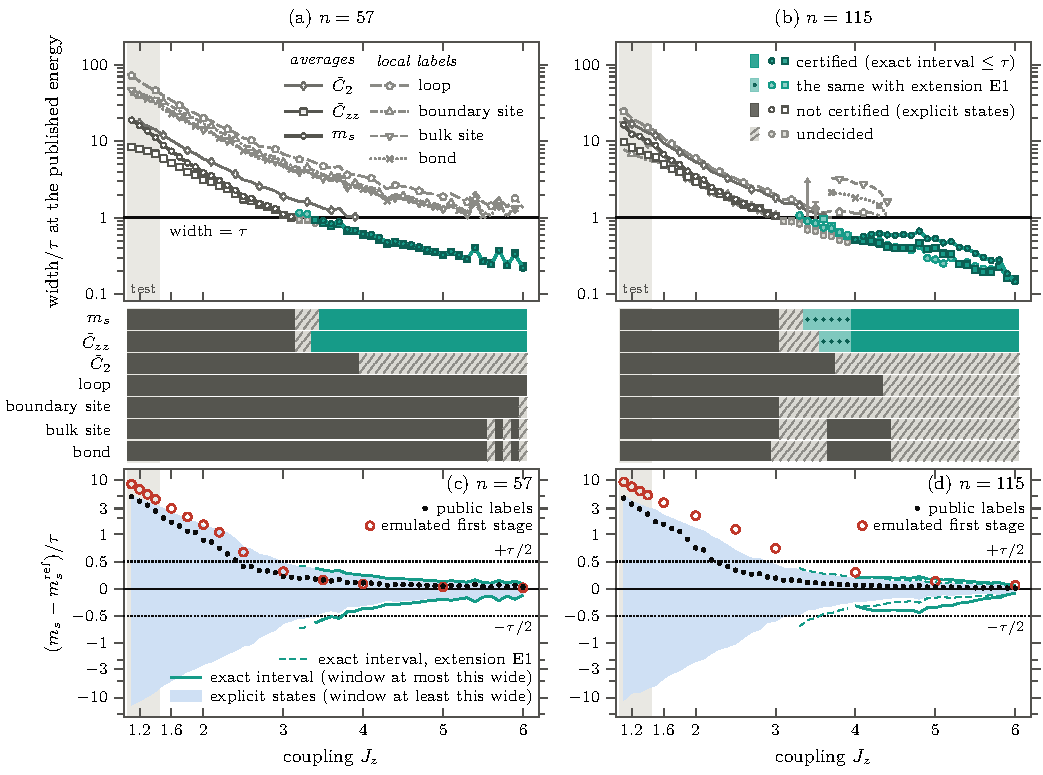
\includegraphics[width=\textwidth]{fig1_map_rd_pgf}%
\caption{\label{fig:map}The certification map at the published energies, and the public labels inside it.
(a, b) Width of each label's interval at the published energy, in units of $\tau=0.06|o_\GS|$ (log scale), at every % src: def:phase3/full_runs/real_data/DECLARATION.md (tau = 0.06 |O_GS|)
coupling of the dataset, for $n=57$ and $115$. Filled symbols: certified (width of the exact interval, at most
$\tau$). Open symbols: not certified (distance between the labels of two explicit states of the window, at least
$\tau$; for $\Ctwo$ and the local labels, grey, one symbol per three couplings). Light grey, for $\ms$ and $\Czz$: undecided
(explicit states less than $\tau$ apart, no exact interval within $\tau$ under the declared rule), with a bar up
to the width of an exact interval where one exists (drawn up to $3\tau$; an arrow marks the one bar cut there, $8.9\,\tau$). % src: file:paper/figures/pgf_map_rd/export_check.txt (exact interval 8.9 tau wide, rounded down; drawn up to 3 tau with an arrow)
Strip under each panel: the status of every label at every
coupling (teal: certified; dark grey: not certified; light grey, hatched: undecided). Every certified status rests on hypothesis H of
Sec.~\ref{sec:dataset} and is the same with the reference-free tolerance; the ``not certified'' statuses do not use
H and use the reference tolerance (Methods).
The order parameter $\ms$ is certified at $26$ of the 45 training couplings at $n=57$ ($\Jz=3.5$--$6.0$) and at $21$ % src: rdq:jstar.57_m_s.sec2.certified_exact (26); rdq:jstar.115_m_s.sec2.certified_exact (21)
at $n=115$ ($\Jz=4.0$--$6.0$), the mean correlation $\Czz$ at $27$ and $21$; no certificate was computed for $\Ctwo$ and the % src: rdq:jstar.57_Czz_bar.sec2.certified_exact (27); rdq:jstar.115_Czz_bar.sec2.certified_exact (21)
local labels. At $n=115$ states aimed at a local label were stored only for the bulk site at $\Jz=4$, and $92$ of % src: file:paper/figures/pgf_map_rd/export_check.txt (92 of the 200 at n = 115)
the $200$ local rows are undecided, against $7$ at $n=57$. Light symbols on dashed lines, and dotted cells: the % src: file:paper/figures/pgf_map_rd/export_check.txt (92 of the 200 at n = 115, 7 of the 200 at n = 57)
extension E1 (declared with the analysis, computed after it), which certifies $27$ ($\ms$) and $25$ ($\Czz$) of the % src: rdeq:jstar.115_m_s.sec2_e1.certified_exact (27); rdeq:jstar.115_Czz_bar.sec2_e1.certified_exact (25)
45 couplings at $n=115$ and none more at $n=57$. Shaded: the four test couplings, where all seven labels are not
certified.
(c, d) The interval of $\ms$ and the public labels (dots), as distances from the reference in units of $\tau$
(scale linear up to $\pm\tau$, logarithmic beyond; band: between the two explicit states; lines: exact interval,
dashed with E1; dotted: $\pm\tau/2$). The public labels lie above the reference at every coupling of both sizes, and
inside the exact interval wherever one exists. The emulated first stage of the method class (circles), at its own energy
(Sec.~\ref{sec:method}; at $n=115$ its energy error is more than $3.8$ times the published one), has the same sign % src: file:paper/figures/pgf_map_rd/export_check.txt (more than 3.8 times)
and the same trend. Drawn from the deposited data by a script written with an AI tool (Methods).}
\end{figure*}

\subsection{The method class inside the window: emulation, public labels, our device}
\label{sec:method}

The map says where energy is silent. To see what a generator does there, we emulated the first stage of the method
class of the dataset~\cite{jaderberg2026,yu2025skqd} classically, with the published time steps and shot budget (Methods): the labels come from
the lowest eigenvector of $H$ in the span of the sampled configurations. At $n=57$ the emulation meets its declared % src: def:phase3/full_runs/map/DECLARATION.md (n = 57)
energy condition, set against the dataset paper's Fig.~2; per site its energy error is $2.2$, $1.9$ and $1.3$ times % src: rdee:sizes.57.rows[Jz=1.6].ratio (2.180); rdee:sizes.57.rows[Jz=2.0].ratio (1.933); rdee:sizes.57.rows[Jz=3.0].ratio (1.349); fig: Ref. [jaderberg2026] Fig. 2
the published final one at $\Jz=1.6$, $2.0$ and $3.0$, so near the isotropic point it probably overstates the bias. At % src: rdee:sizes.57.rows[Jz=3.0].ratio (1.349)
$n=115$ it does not: its energy error at the published budget is $3.82$--$5.94$ times the % src: rdee:sizes.115.ratio_min (3.825); rdee:sizes.115.ratio_max (5.937); derived: range rounded outward, 3.8250 floored to 3.82 and 5.9369 ceiled to 5.94
published final one, so $n=115$ emulation numbers describe the method class at that budget only. The emulation
omits the final basis-optimization step. Built as the dataset paper's text and diagram describe it, with the rotation
on the target qubit of each pair of CNOTs, that step gave no energy gain in our emulation. The authors'
code~\cite{jaderberg2026data}, which we read and did not run, puts the rotation on the control qubit, one angle per
edge (the optimized angles are not public), and evaluates the labels in the rotated state; this block is one of two
variants we had built before we knew the code, and in our emulation it reproduces the reported gain and leaves the
bias-versus-energy relation unchanged. The order and orientation of the CNOTs and the optimizer were not compared (Supplemental
Sec.~S5). The emulated first stage, with its $1\%$ bit flips, has $0.10$--$0.59$ ($n=57$) and $0.05$--$0.59$ % src: def:phase3/full_runs/method/DECLARATION.md (1 % floor); file:phase3/full_runs/real_data/checks/r11/fp_hostileB_extra_checks_out.txt (0.103 to 0.581; 0.059 to 0.581); derived: ranges rounded outward
($n=115$) times the energy error per site of the dataset's own, which the public files hold; the final step lowers % src: def:phase3/full_runs/real_data/DECLARATION.md (n = 115)
that error $2.8$--$8.9$ and $6.6$--$175$ times, so in energy the emulation lies between the dataset's two stages % src: rdp:post_hoc.per_size.57.de_first_over_de_real.min (2.80); rdp:post_hoc.per_size.57.de_first_over_de_real.max (8.93); rdp:post_hoc.per_size.115.de_first_over_de_real.min (6.59); rdp:post_hoc.per_size.115.de_first_over_de_real.max (175.4)
at $n=115$ and, at $n=57$, up to $\Jz=3.0$, and below both from $\Jz=3.5$. % src: file:phase3/full_runs/real_data/checks/r11/fp_hostileB_extra_checks_out.txt (emu/final 1.349 at 3.0, 0.998 at 3.5)

\emph{A one-sided bias in the emulation.} At $n=57$, $\Jz=1.2$, the emulated states carry $\ms$ larger than % src: emu(57,1.2):var.primary.err.dm_s (0.2586)
the reference by $+0.259$; every site is more ordered, every correlation stronger and every loop larger, in all % src: emu(57,1.2):var.primary.err.dm_s (0.2586)
$147$ states we checked, at every $\Jz$ and both sizes. The bias % src: file:phase3/full_runs/method/RESULTS.md (147); file:phase3/full_runs/real_data/checks/r11/fp_counts_out.txt (103 + 44 = 147)
falls with $\Jz$: $+0.139$ at $1.6$, $+0.036$ at $2.5$, $+0.005$ at $4.0$ [circles in Fig.~\ref{fig:map}(c), there in units of $\tau$]. It is created by % src: emu(57,1.6):var.primary.err.dm_s (0.1390); emu(57,2.5):var.primary.err.dm_s (0.0364); emu(57,4.0):var.primary.err.dm_s (0.0050); def:phase3/full_runs/method/DECLARATION.md (Jz grid 1.6, 2.5, 4.0)
the diagonalization in a truncated configuration set: perfect samples of the DMRG ground state, cut to the same
subspace dimension, reproduce it, while their multiplicity-weighted mean is unbiased; it falls only slowly with
that dimension (Supplemental Sec.~S5 and Sec.~S12). The sign is a property of this model
and regime, not of the method class: on the benchmark of Sec.~\ref{sec:bench} the same truncation weakens order.

\emph{The same bias in the public labels.} The dataset's own labels show this sign and this trend, as a measurement
against the authors' DMRG reference (Methods). Every one of the $100$ published values of $\ms$ ($50$ couplings, two sizes) is more % src: rdp:sizes.57.n_couplings (50); derived: 2 x 50 = 100 values, all with a positive miss (rdp:sizes.<n>.P5.rows, Delta > 0)
ordered than the reference: by $4.95\,\tau$ at $\Jz=1.1$ and $0.04\,\tau$ at $6.0$ for $n=57$, and by $4.67\,\tau$ % src: rdp:sizes.57.P4.m_s.D.1.1 (4.954); rdp:sizes.57.P4.m_s.D.6.0 (0.0374); rdp:sizes.115.P4.m_s.D.1.1 (4.667)
at $1.1$ for $n=115$. Taken one by one, $32\,785$ of the $32\,800$ pairs of a published label and its reference % src: rdap:G.total (32785, 32800); file:phase3/full_runs/real_data/RESULTS.md (32,785 of 32,800 pairs)
(sites, nearest- and second-neighbour correlations and loops, at both sizes) lie on the N\'eel side of the
reference, and the error falls with the coupling: its rank correlation with $\Jz$ lies between $-0.996$ and % src: rdp:sizes.115.P4.sites.spearman (-0.9955); derived: -0.99549 rounded outward to -0.996 (lesson 7b)
$-0.971$ in the eight cases ($50$ couplings each). Sign and trend were tests fixed in writing before they ran, after an initial look at % src: rdp:sizes.57.P4.loops.spearman (-0.9720); derived: -0.97196 rounded outward to -0.971 (lesson 7b); rdp:sizes.57.n_couplings (50)
the data that had already shown them for $\ms$ (Methods; exceptions in Supplemental Sec.~S18). The
public labels come after the final optimization, and at equal coupling their bias is smaller than that of the
emulation: $+0.077$ against $+0.139$ at $n=57$, $\Jz=1.6$. % src: rdp:sizes.57.P5.rows[Jz=1.6].Delta (0.0771); emu(57,1.6):var.primary.err.dm_s (0.1390)

\emph{Our device.} We ran the same first stage on a superconducting heavy-hex processor at $n=57$, a single run per % src: def:phase3/full_runs/map/DECLARATION.md (n = 57)
coupling (Methods). At $\Jz=1.2$ the
device labels over-order all 57 sites and every nearest-neighbour correlation, with $\Delta\ms=+0.310$ % src: qpu:points.1.2.device.rec.dm_s (0.3098); file:phase3/full_runs/qpu/RESULTS.md (57/57)
[Fig.~\ref{fig:landscape}(c)]; the noiseless simulation of the identical circuits gives $+0.253$, so in this run the % src: qpu:points.1.2.control.rec.dm_s (0.2527)
truncation creates most of the bias and the device noise adds $+0.057$ (one job, not repeated). At $\Jz=1.6$ and $4.0$ the device gives $+0.196$ and % src: qpu:points.1.2.D3_dm_s_device_minus_control (0.0572); qpu:points.1.6.device.rec.dm_s (0.1955)
$+0.024$ with fewer shots, again at every site, though at $4.0$ the smallest site excess, $+0.013$, is not resolved % src: qpu:points.4.0.device.rec.dm_s (0.0239); qpu:points.4.0.device.rec.signed_dZ_min (0.0134); file:phase3/full_runs/qpu/RESULTS.md (4.0)
against the unmeasured run-to-run variation. These device states lie in the sector, and at none of the three
couplings is the energy low enough for the sector window to certify $\ms$ (Supplemental Sec.~S6). For one of them the
interval is proved with no reference value: at $\Jz=4.0$ the energy of the device vector in exact arithmetic and stored
lower bounds give $\ms\in[0.868,0.997]$ and $\Czz\in[-0.996,-0.887]$, which contain the labels but are $2.5$ and $2.0$ % src: ftc:C1.rec.m_s.lo (0.8684); ftc:C1.rec.m_s.hi (0.9969); ftc:C1.rec.Czz_bar.lo (-0.9951); ftc:C1.rec.Czz_bar.hi (-0.8879); ftc:C1.rec.m_s.w_over_tau (2.466); ftc:C1.rec.Czz_bar.w_over_tau (2.011); derived: end points rounded outward (-0.99508 -> -0.996, -0.88794 -> -0.887; lesson 7b)
times wider than $\tau$ (Methods; for $\Jz=6.0$ see Sec.~\ref{sec:predict}). Signed loops and % src: file:phase3/full_runs/final_tests/RESULTS.md (6.0)
next-nearest-neighbour correlations were not analysed on the device.

\section{The bias against the energy}
\label{sec:predict}

\begin{figure*}[t]
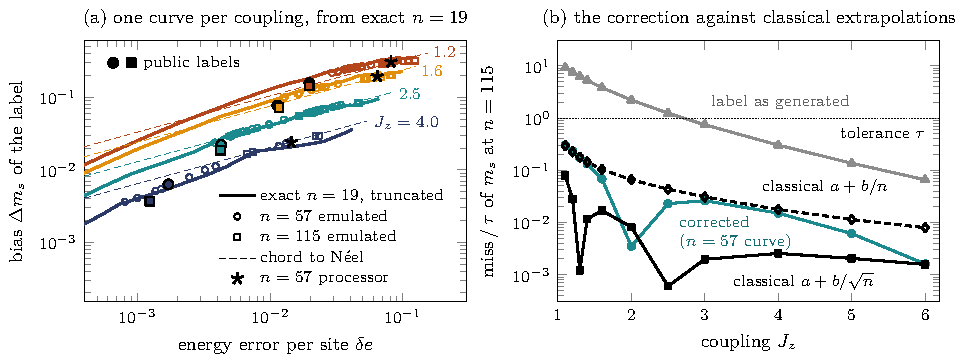
\includegraphics[width=\textwidth]{fig_bias_law_rd}%
\caption{\label{fig:biaslaw}The bias against the energy (exploratory data, with the public labels added; the declared tests are in Sec.~\ref{sec:predict}).
(a) Bias of $\ms$ against the energy error per site at four couplings. Solid lines: the exact ground state at $n=19$, % src: file:phase3/full_runs/bias_law/code/bias_law.py (n = 19)
truncated to its most probable configurations. Dashed lines: the parameter-free chord between the ground state and the
N\'eel state at $n=19$. Open symbols: the stored emulated states at $n=57$ and $115$ (pipeline variants with and without % src: def:phase3/full_runs/map/DECLARATION.md (57, 115)
noise, shot scans, subsets of perfect samples); stars: our device labels. Filled symbols: the public labels at their
published energy errors (circles: $n=57$; squares: $n=115$). Seven of these eight labels have between $0.69$ and % src: rdp:sizes.115.P5.rows[Jz=2.5].ratio (0.6962); derived: lower end floored (lesson 7b)
$0.86$ of the bias that the curve of their coupling gives at the same energy error; the eighth ($n=57$, $\Jz=4.0$) % src: rdp:sizes.57.P5.rows[Jz=1.2].ratio (0.8558)
has $1.15$ times that bias. The declared test of the curve on the public labels, at all 50 couplings, fails at % src: rdp:sizes.57.P5.rows[Jz=4.0].ratio (1.1502); rdp:sizes.115.P5.all.n_couplings (50)
$n=115$: $12$ of the $19$ ratios that decide it lie below the declared band (Sec.~\ref{sec:predict}). Colours mark % src: rdp:P5_rule.ratios_outside_115 (12 couplings); rdp:sizes.115.P5.all.n_deciding (19)
the coupling, written at the end of each curve; the legend, in black, shows the kind of data.
(b) The emulated label at $n=115$: miss of $\ms$ of the label as generated, of the label corrected with the curve of the $n=57$ emulation, and of % src: def:phase3/full_runs/map/DECLARATION.md (57, 115)
two classical extrapolations of the truth from $n=19$ and $57$ that use no quantum data. The dip of the corrected label % src: file:phase3/full_runs/bias_law/code/bias_law.py (n = 19, 57)
near $\Jz=2$ is a change of sign of its residual, not a gain in accuracy. % (coupling read from the figure)
Drawn from the deposited data by a script written with an AI tool (Methods).}
\end{figure*}

The window of Sec.~\ref{sec:setting} holds for every state at a given energy, whereas a generator follows one path through
it. This section looks at that path: a curve of the bias against the energy error, found by exploration on the emulated
first stage after its data were in hand, and then four tests whose rules we fixed in writing before running them.
Except for the last, which proves an interval, none of it is a certificate.

\emph{One curve per coupling.} At $n=19$ we took the exact ground state at each $\Jz$, kept its $D$ most probable % src: file:phase3/full_runs/bias_law/code/bias_law.py (n = 19)
configurations and diagonalized $H$ in their span, for a grid of $D$: a curve of the bias $\Delta\ms$ against $\de$
that uses no emulator and no device. The $127$ stored emulated states at the four couplings of Fig.~\ref{fig:biaslaw}(a) lie within % src: file:phase3/full_runs/real_data/checks/r11/fp_bias_curve_recompute_out.txt (127 states)
$-13$ to $+25\%$ of that curve and our six device readings (three couplings, each with and without recovery) % src: blw:nulls.spread_pct_low (12.39); blw:nulls.spread_pct_high (24.32); derived: ranges rounded outward, 12.39 to 13, 24.32 to 25 (lesson 7b)
within $-9$ to $+18\%$ (over all stored couplings: $-13$ % src: file:phase3/full_runs/real_data/checks/r11/fp_bias_curve_recompute_out.txt (-8.7 % .. +17.1 %; -12.65 % .. +41.22 %); derived: ranges rounded outward, 8.7 to 9, 17.1 to 18, 12.65 to 13 (lesson 7b)
to $+42\%$, the upper end where the bias is at most $0.3\,\tau$). Subtracting the bias read off the curve at each % src: file:phase3/full_runs/real_data/checks/r11/fp_bias_curve_recompute_out.txt (ratio 1.4122; raw=0.293 tau); derived: 41.22 rounded up to 42 and 0.293 to 0.3
label's own $\de$ lowers the mean miss of $\ms$ from $2.4$ to $0.06\,\tau$ at $n=57$ (at most $0.18\,\tau$) and from % src: blw:n19_curve.57.raw.mean (2.43); blw:n19_curve.57.corrected.mean (0.062); blw:n19_curve.57.corrected.max (0.1737); derived: 0.1737 rounded up to 0.18
$3.4$ to $0.39\,\tau$ at $n=115$ ($0.70$--$0.97\,\tau$ at the four test couplings), against $0.59$ and $0.88\,\tau$ % src: blw:n19_curve.115.raw.mean (3.36); blw:n19_curve.115.corrected.mean (0.385); blw:nulls.n19_curve_115_test_min (0.701); blw:nulls.n19_curve_115_test_max (0.971); blw:n19_curve.57.small_truth.mean (0.585); blw:n19_curve.115.small_truth.mean (0.883)
for quoting the exact value at $n=19$, and from $4.3$ to $0.34\,\tau$ for our device labels (at most $0.78\,\tau$). % src: blw:device.raw.mean (4.27); blw:device.n19.mean (0.338); blw:device.n19.max (0.7709); derived: 0.7709 rounded up to 0.78

\emph{What is generic.} Much of this reduction is forced by the endpoints: every state here lies between the ground
state and the N\'eel state, and a parameter-free chord $(1-m_s^{\rm GS})\sqrt{\de/\de_{\text{N\'eel}}}$ from the
$n=19$ ground state alone gives mean misses of $0.37$, $0.11$ and $0.12\,\tau$ at $n=57$, at $n=115$ and on the % src: blw:nulls.chord_57.mean (0.367); blw:nulls.chord_115.mean (0.105); blw:nulls.chord_device.mean (0.124)
device (at most $1.4$, $0.28$ and $0.31\,\tau$), better than the truncated curve in the last two cases. Both readings % src: blw:nulls.chord_57.max (1.386); blw:nulls.chord_115.max (0.2718); blw:nulls.chord_device.max (0.3033); derived: maxima rounded up, 0.2718 to 0.28 and 0.3033 to 0.31
need $\de$, hence $E_0$, at the target size; we do not claim that a small exact calculation suffices (Supplemental
Sec.~S13).

\emph{Origin.} For a fixed set of configurations and a small weight outside it, the bias of a diagonal label is
linear in the energy error~\cite{white2007}; most of our data lie outside that limit, and we have no derivation
of the transfer across sizes (Supplemental Sec.~S13, with internal checks of a biased family that did not reveal
the bias). We did not find the same curve reported across sizes, nor a correction of the labels of sample-based
diagonalization, where corrections so far act on the energy~\cite{raisuddin2025}.

\emph{Limits.} The curve belongs to one stage of one method class: on the public labels its ratios stay inside the
declared band at $n=57$ and it overstates the bias at $n=115$, so its declared test fails (below). It is not
universal: on three other models at $n=20$ the corrected value beats the % src: file:phase3/full_runs/bias_law/inputs/generality.txt (20)
exact value of the smaller system in all $8$ combinations at strong order and in $1$ of $14$ near the isotropic point % src: blw:other_models.wins_strong (8); blw:other_models.n_strong (8); blw:other_models.wins_hard (1); blw:other_models.n_hard (14)
or with frustration or disorder (Supplemental Sec.~S13). Most important, classical
two-point extrapolations of the reference values at $n=19$ and $57$ miss $\ms$ at $n=115$ by $0.10$, $0.04$ and % src: blw:nulls.a_b_over_n.mean (0.102); blw:nulls.a_b_edges_over_n.mean (0.037)
$0.01\,\tau$ on average (forms $a+b/n$, $a+b\,N_e/n$ with $N_e$ edges, and $a+b/\sqrt n$), and the label corrected % src: blw:nulls.a_b_over_sqrt_n.mean (0.014)
with the $n=57$ curve by $0.09\,\tau$ [Fig.~\ref{fig:biaslaw}(b)]: it matches the simplest form and does not reach the % src: blw:classical_tie_115.corr57.mean (0.090)
other two: on this uniform model the curve tells how large a label's error is likely to be and does not recover
information that a classical calculation lacks.

\emph{Declared tests.} We then fixed four tests in writing, their rules checksummed before the computations started
(Methods; Supplemental Sec.~S14 and Sec.~S18). One applies the recipe of the $n=19$ curve, unchanged, to emulated
labels at seven new couplings that lie between those explored ($\Jz=1.5$ to $3.2$). The rule, written with the % src: def:phase3/full_runs/final_tests/DECLARATION.md (1.5, 1.7, 2.8, 3.2)
exploratory values in hand, asked for mean misses of at most $0.2$ ($n=57$) and $0.6\,\tau$ ($n=115$) and for every % src: fta:rule.limit57 (0.2); fta:rule.limit115 (0.6)
ratio of the bias to the curve to lie in $[0.75,1.3]$. The curve passes: the mean miss falls from $1.7$ to % src: def:phase3/full_runs/final_tests/DECLARATION.md (0.75, 1.3); fta:summary.57.raw.mean (1.704)
$0.06\,\tau$ and from $2.9$ to $0.34\,\tau$ (greatest single miss $0.14$ and $0.59\,\tau$), with ratios of % src: fta:summary.57.miss_curve19.mean (0.0619); fta:summary.115.raw.mean (2.904); fta:summary.115.miss_curve19.mean (0.3398); fta:summary.57.miss_curve19.max (0.1322); fta:summary.115.miss_curve19.max (0.5840); derived: maxima rounded up, 0.1322 to 0.14 and 0.5840 to 0.59
$0.88$--$1.06$. Linear interpolation of the exploratory misses gives $0.06$ and $0.35\,\tau$ and so predicted this % src: fta:rule.ratio_min (0.8849); fta:rule.ratio_max (1.0568); ftp:interp_mean.57 (0.0635); ftp:interp_mean.115 (0.3511)
outcome: the test probes only surprises between grid points, on the same lattice and pipeline.

\emph{The curve on the public labels.} A second test applies the same recipe and rule to the public labels at all
$50$ couplings of each size, the curve being read at each label's published energy. It was fixed after an initial % src: rdp:sizes.57.n_couplings (50)
look at the data, which had shown the bias and the energy errors but no ratio between them (Methods). Subtracting the
curve lowers the mean miss of $\ms$ from $0.62$ to $0.11\,\tau$ at $n=57$ and from $0.53$ to $0.17\,\tau$ at % src: rdp:sizes.57.P5.all.mean_raw_miss_tau (0.623); rdp:sizes.57.P5.all.mean_miss_tau (0.111); rdp:sizes.115.P5.all.mean_raw_miss_tau (0.530); rdp:sizes.115.P5.all.mean_miss_tau (0.168)
$n=115$, inside both declared limits ($0.2$ and $0.6\,\tau$; the uncorrected labels already met the second). % src: rdp:sizes.57.P5.all.mean_miss_limit (0.2); rdp:sizes.115.P5.all.mean_miss_limit (0.6)
The test nevertheless fails, on its second condition: at $n=57$ all $22$ % src: rdp:sizes.57.P5.all.n_deciding (22)
ratios that decide (labels that miss by at least $0.2\,\tau$) lie in the band, from $0.80$ to $1.05$, but at % src: def:phase3/full_runs/real_data/DECLARATION.md (raw miss is at least 0.2 tau); rdp:sizes.57.P5.all.ratio_range_deciding (0.8029, 1.0455)
$n=115$, $12$ of the $19$ lie below it (from $0.60$ to $0.82$, median $0.74$). There the public bias is about a % src: rdp:P5_rule.ratios_outside_115 (12 couplings); rdp:sizes.115.P5.all.n_deciding (19); rdp:sizes.115.P5.all.ratio_range_deciding (0.6087, 0.8122); derived: range rounded outward, 0.6087 to 0.60 and 0.8122 to 0.82; rdp:post_hoc.per_size.115.ratio_median_deciding (0.741)
quarter smaller than the curve of the first stage, and by the rule written beforehand the curve stays restricted to
that stage. The chord leaves less, $0.058$ and $0.094\,\tau$ (both readings take $E_0$ from DMRG here). % src: rdp:sizes.57.P5.all.mean_miss_chord_tau (0.0584); rdp:sizes.115.P5.all.mean_miss_chord_tau (0.0937)
Quoting the exact $19$-site value needs neither $E_0$ nor the label and misses by $0.29$ and $0.41\,\tau$ on % src: rdp:sizes.57.P5.all.mean_miss_n19_truth_tau (0.294); rdp:sizes.115.P5.all.mean_miss_n19_truth_tau (0.407)
average (more at the test couplings, Supplemental Sec.~S18): more than either corrected label, less
than the label as published.

\emph{Disordered lattices.} A third test asks whether corrected labels beat local classical estimates where no
uniform extrapolation applies: six instances at each of $\Jz=1.6$ and $2.5$ at $n=57$, every bond scaled by a factor % src: def:phase3/full_runs/final_tests/DECLARATION.md (1.6, 2.5)
drawn uniformly from $[0.5,1.5]$, $121$ site and bond labels per instance, DMRG references, and learned models % src: def:phase3/full_runs/final_tests/DECLARATION.md (0.5, 1.5, 121)
trained on disordered $n=19$ instances only. The
quantum estimate is the emulated label plus a learned correction; the classical estimates use no quantum data, and the
best of six was chosen after the fact, which favours them. The rule asked the quantum estimate to be at least $25\%$ % src: def:phase3/full_runs/final_tests/DECLARATION.md (0.25); derived: 0.25 = 25 %
better than the best classical one and to win in five of six instances, at both couplings. It does not
(table in Supplemental Sec.~S14): the correction lowers the miss about four times, but a $19$-site cluster with a mean-field
boundary is $9$ and $21$ times closer to the reference than the corrected label ($7.0$--$10.1$ and $19.6$--$23.3$ times in the single % src: ftp:ratio_to_best_1.6.q_top (9.06); ftp:ratio_to_best_2.5.q_top (21.06); file:paper/reviews/R10_2026-11-12/scratch/phys-declared-stats/recompute_table2_out.txt (min 7.09 max 10.08; min 19.65 max 23.29); derived: ranges rounded outward
instances), in all $12$ instances, and DMRG on the target at bond dimension $32$, about a minute per instance, does % src: fts:test_b_instances_total (12); def:phase3/full_runs/final_tests/DECLARATION.md (32); fts:minutes_per_instance.dmrg32 (0.83, 1.06)
better still (a possible reason, the locality of gapped ground states, is discussed in Supplemental Sec.~S14; we
did not measure the gap of these instances). Against a regression on the same local
couplings, a comparison added after the outcome was known, the label helps in the mean: the miss falls by $19\%$ and % src: ftp:gain_over_reg_1.6.q_top (19.4)
$14\%$, in $4$ of $6$ and $6$ of $6$ instances. This regime, which DMRG solves, says what labels add where classical % src: ftp:gain_over_reg_2.5.q_top (13.8); file:paper/reviews/R10_2026-11-12/scratch/phys-declared-stats/recompute_table2_out.txt (wins 4/6; wins 6/6)
methods work, not where they fail; the untested cases and all estimates are in Supplemental Sec.~S14.

\emph{A processor label.} A fourth test asked for one processor label with a proved interval below $\tau$ (at
$\Jz=4.0$ it is wider, Sec.~\ref{sec:method}). The run at $\Jz=6.0$ was not submitted % src: file:phase3/full_runs/qpu/RESULTS.md (4.0); file:phase3/full_runs/final_tests/RESULTS.md (6.0)
on the day of the other tests, a departure from the declared procedure; it was submitted two days later, under added
conditions that could stop it but not cause it, ran on 2026-11-10, and both bit-order checks passed (Methods). % src: file:phase3/full_runs/final_tests/RESULTS.md (2026-11-10)
With no reference value, the label's $\ms$ lies in a proved interval $0.50\,\tau$ wide ($\Czz$: $0.57\,\tau$), so for % src: ft3:C3.rec.m_s.w_over_tau (0.4992); derived: 0.4992 ceiled to 0.50 (a width that bounds the distance); ft3:C3.rec.Czz_bar.w_over_tau (0.5678)
this one label, at this one coupling, the distance to the ground-state value is proved to be at most that width. A
classical energy gives a narrower interval here ($0.12\,\tau$). % src: ftx:intervals.dmrg_E0.m_s.w_over_tau (0.1232)

\emph{What the energy says where it certifies nothing.} For this method class and this model the answer is
modest: the energy error per site estimates the size of the label error, within the limits listed above, and
corrected labels did not improve on classical estimates.



\section{What a learner can guarantee}
\label{sec:learn}

The dataset paper names the dependence of learned models on ``system size, observable locality, and proximity to
phase boundaries'' as a direction for future work~\cite{jaderberg2026}; the rule above addresses the part of that question
that concerns the labels. The windows of
Sec.~\ref{sec:setting} give every training label $y_i=y(x_i)$ an energy interval $I_i=[\ell_i,h_i]$, computed from its
energy (Lemma~\ref{lem:dual}; for the public labels of Sec.~\ref{sec:dataset}, from the published energy and mean
magnetization), that contains both $y_i$ and the true value $y_i^*$. The following statements, which are
elementary, say what such intervals give a learner. Part (b) is split conformal prediction with each calibration
score replaced by its greatest value over the label's interval, the pessimistic score of
Ref.~\cite{javanmardi2023} for set-valued labels, with the same proof of validity. In the terms of
Ref.~\cite{cauchois2022} it obtains strong coverage from weak labels, at a price in width that that work bounds
from below and part (d) makes explicit. What the
physics adds is the interval: it is per
label, computed from that label's own energy without access to the truth, and its width is known in advance
from Sec.~\ref{sec:rule}. Parts (b)--(d) hold for any learner, including neural networks; only (a) uses linearity.

\begin{proposition}[Learning from label intervals]
\label{prop:learn}
Let the inputs $x$ be exchangeable, the true label $y^*(x)$ a function of $x$, and every training and calibration
label come with an interval $I(x)=[\ell(x),h(x)]\ni y^*(x),\,y(x)$ of width $w(x)$.
(a) For a learner linear in its training labels, $f(x)=\sum_i a_i(x)\,y_i$ with label-independent coefficients, and
$f^*$ the same learner trained on the true labels, $|f(x)-f^*(x)|\le W(x)\equiv\sum_i|a_i(x)|\,w_i$ for
every $x$, in or out of distribution.
(b) Let $f$ be trained on separate data, $s_j=\max_{y\in I_j}|f(x_j)-y|$ the scores of $m$ calibration inputs, and
$q$ the $k$-th smallest of them, $k=\lceil(m+1)(1-\alpha)\rceil$ ($q=+\infty$ if $k>m$). Then a new input,
exchangeable with the calibration inputs, satisfies $P(|f(x)-y^*(x)|\le q)\ge1-\alpha$, whatever the generator's bias.
(c) If $P(y^*(x)\in C(x))\ge1-\alpha$, the rule ``answer the midpoint $c(x)$ of $C(x)$ if and only if
$|C(x)|\le\tau$'' gives $P(\text{answered and }|c(x)-y^*(x)|>\tau/2)\le\alpha$, so the error rate among answers is
at most $\alpha$ divided by the answer rate.
(d) In (b), whatever the learner, $2q\ge w_{(k)}$, the $k$-th smallest of the widths $w_j$ of the calibration
intervals, with equality when $f(x_j)$ is the midpoint of $I_j$ for every $j$.
\end{proposition}

\noindent\emph{Proof sketch.} (b) $s_j\ge|f(x_j)-y_j^*|$, so $q$ is at least the conformal quantile of the
true-label scores. (d) $s_j\ge w_j/2$, half the width of $I_j$. Full proofs: Supplemental Sec.~S8. $\square$

Standard split conformal prediction~\cite{angelopoulos2021} uses the scores $|f(x_j)-y_j|$ and covers $y(x)$, not
$y^*(x)$; we call the intervals of (b) \emph{energy-calibrated}. Rule (c) with the
intervals of (b) is the learner-side rule; these intervals have the same width at every input, so it decides per
label. Part (d) is its floor and says what a guarantee below the tolerance needs: the rule can answer only if at
least $k$ of the $m$ calibration labels have energy intervals no wider than the tolerance, whatever the learner and
whatever labels it was trained on. For other scores the floor is the query's own energy interval: when the query
comes with an energy interval that is exchangeable with those of the calibration labels, the returned set contains
it with probability at least $1-\alpha$; a remark after Ref.~\cite{cauchois2022} extends this to
every procedure whose guarantee rests on the energies alone (Supplemental Sec.~S8). A simpler rule filters labels:
\emph{answer at an input only if the generated label there is certified at its own energy}. It needs a generated
label and its energy at the query, as a test set has; its price is the width of the energy intervals, which
Sec.~\ref{sec:rule} predicts before any training.

\subsection{The public labels at 57 and 115 qubits}
\label{sec:realistic}

The public labels of Sec.~\ref{sec:dataset}, their energies and the authors' own DMRG
reference~\cite{jaderberg2026data} allow the statements above to be
tested on the labels themselves, with that reference as the truth. The dataset paper measures its models against
the processor's labels and reports the errors of the labels against DMRG separately; the tests below ask what
agreement with the labels says about the error against DMRG. The tests and their pass rules were fixed in
writing before they were run, after an initial look at the data that included the energies and the labels of $\ms$
against their reference but no learning result (Methods); $n=57$ decides and $n=115$ is reported. % (sizes)

\emph{Protocol.} Per-site regressors of $\langle Z_i\rangle$ are trained on the public labels of the training range
and $\ms$ is derived from them, as in the dataset paper. The primary model is a cubic in $1/\Jz$, which is linear in
its labels. Standard intervals at nominal level $0.9$ are calibrated on held-out public labels, each % src: rdl:sealed.results_cheap.alpha (0.1); derived: 1 - alpha
training coupling being held out in turn: the plain jackknife, which has no finite-sample guarantee~\cite{barber2019},
on a fixed grid of couplings. With the jackknife+ of Ref.~\cite{barber2019}, whose level under exchangeability is
$1-2\alpha$, the counts below are the same at $n=57$ and are $41$ labels and $11$ truths at $n=115$ (post hoc). % src: file:phase3/full_runs/real_data/checks/r11/fl_learn_paper_numbers_out.txt (jackknife+: 41 labels and 0 truths of 45 at n = 57; 41 labels and 11 truths of 45 at n = 115)
As a control, the same model is trained and calibrated on the DMRG
labels, so that model error and label error can be separated. Widths and misses are in units of the tolerance
$\tau=0.06|o_\GS|$ at each coupling. % src: rdl:sealed.results_cheap.tau_rel (0.06)

\emph{Standard intervals follow the labels} [Fig.~\ref{fig:overview}(c)]. In the training range at $n=57$ the % (sizes)
intervals, $0.09$--$0.15\,\tau$ wide, contain $41$ of the $45$ held-out public labels, at the nominal rate, and the true % src: rdl:summary.57.models.poly3_invJ.real.ind.width_tau (0.0966, 0.1496); file:phase3/full_runs/real_data/results/RESULTS_learn.md (0.096-0.150, rounded outward); rdl:summary.57.models.poly3_invJ.real.ind.label_covered (41)
$\ms$ at none of the $45$ couplings. The held-out prediction misses it by $0.05$--$1.64\,\tau$ (median $0.12\,\tau$): % src: rdl:summary.57.models.poly3_invJ.real.ind.truth_covered (0); rdl:summary.57.models.poly3_invJ.real.ind.miss_tau (0.0529, 1.6395); file:phase3/full_runs/real_data/checks/r11/fl_learn_paper_numbers_out.txt (miss 0.05-1.64 tau, range rounded outward; median 0.12 tau)
by more than $\tau$ at $\Jz=1.6$--$1.9$, by more than $\tau/2$ at $\Jz=1.6$--$2.4$ and by at most $0.16\,\tau$ from $\Jz=3.5$, % src: file:phase3/full_runs/real_data/checks/r11/fl_learn_paper_numbers_out.txt (miss above tau at 4 couplings: Jz = 1.6-1.9; above tau/2 at 9 couplings: Jz = 1.6-2.4; from Jz = 3.5 at most 0.16 tau, rounded up from 0.1565)
where the truth lies just outside intervals a tenth of the tolerance wide. At $n=115$ they contain $40$ of the labels and the truth at the $11$ couplings $\Jz=5.0$--$6.0$. % src: rdl:summary.115.models.poly3_invJ.real.ind.label_covered (40); rdl:summary.115.models.poly3_invJ.real.ind.truth_covered (11); file:phase3/full_runs/real_data/checks/r11/fl_learn_paper_numbers_out.txt (truth inside at: Jz = 5.0-6.0, 11 couplings)
With DMRG labels the same pipeline contains the truth at $41$ of the $45$ couplings at both sizes: the intervals % src: rdl:summary.57.models.poly3_invJ.control.ind.truth_covered (41); rdl:summary.115.models.poly3_invJ.control.ind.truth_covered (41)
cover the labels they were calibrated on, and those labels carry the over-ordering
(Sec.~\ref{sec:predict}), which the model reproduces. In the test range the intervals contain the truth at none of the four couplings, at either size,
but neither do those of the control, as no method has a guarantee under a shift of the input: zero coverage there
does not by itself show a label bias. The size of the miss does: $2.28$--$3.73\,\tau$ with the public labels % src: rdl:summary.57.models.poly3_invJ.real.test.miss_tau (2.2860, 3.7202); file:phase3/full_runs/real_data/results/RESULTS_learn.md (2.28-3.73, rounded outward)
($2.37$--$5.07\,\tau$ at $n=115$) against at most $0.25\,\tau$ with DMRG labels, so it is label error, not model % src: rdl:summary.115.models.poly3_invJ.real.test.miss_tau (2.3756, 5.0643); file:phase3/full_runs/real_data/results/RESULTS_learn.md (2.37-5.07, rounded outward; 0.02-0.25); rdl:summary.57.models.poly3_invJ.control.test.miss_tau (0.2425)
error. The same follows for any model that reproduces the labels, with no model run: the dataset paper reports
that its networks reproduce the processor's $\ms$ to better than $3\%$ at the test couplings, where the public labels lie % src: file:phase3/full_runs/real_data/checks/r11/fl_learn_paper_numbers_out.txt (a model within 3 % of the label)
$16.1$--$29.8\%$ ($n=57$) and $14.2$--$28.1\%$ ($n=115$) above its DMRG values, so such a model is at least $2.10\,\tau$ % src: file:phase3/full_runs/real_data/checks/r11/fl_learn_paper_numbers_out.txt (labels 16.1-29.8 % and 14.2-28.1 % above the DMRG values, ranges rounded outward; at least 2.10 tau, rounded down from 2.1087)
and $1.80\,\tau$ above the reference at each of them. % src: file:phase3/full_runs/real_data/checks/r11/fl_learn_paper_numbers_out.txt (at least 1.80 tau, rounded down from 1.8002)
A small neural network, run after the primary result, shows the same pattern in
weaker form, because its intervals are wider: at $n=57$ they % (sizes)
contain $40$ of the $45$ held-out public labels and the truth at $20$ couplings ($n=115$: $42$ and $16$; with % src: file:phase3/full_runs/real_data/checks/r11/fl_neural_f1_out.txt (held-out public labels inside 40 of 45 ; truth inside 20 of 45; inside 42 of 45 ; truth inside 16 of 45)
DMRG labels the truth at $39$ and $43$), and at the test couplings it misses by $2.65$--$6.42\,\tau$ % src: file:phase3/full_runs/real_data/checks/r11/fl_neural_f1_out.txt (truth inside 39 of 45; truth inside 43 of 45); rdl:summary.57.models.mlp_pilot3.real.test.miss_tau (2.6547, 6.4192)
($2.54$--$5.82\,\tau$) with public labels and still by $0.27$--$2.41\,\tau$ ($0.25$--$2.23\,\tau$) with DMRG % src: file:phase3/full_runs/real_data/checks/r11/fl_neural_f1_out.txt (PRINTED 2.54-5.82; PRINTED 0.25-2.23); rdl:summary.57.models.mlp_pilot3.control.test.miss_tau (0.2732, 2.4072)
labels; our implementation of the dataset paper's architecture~1, at $n=57$, by $2.92$--$5.96\,\tau$ and % src: file:phase3/full_runs/real_data/checks/r11/fl_neural_f1_out.txt (architecture 1; n = 57; PRINTED 2.92-5.96)
$0.85$--$2.74\,\tau$ (details: Supplemental Sec.~S19). % src: file:phase3/full_runs/real_data/checks/r11/fl_neural_f1_out.txt (PRINTED 0.85-2.74)

\emph{A label filter.} Keeping a public label only if it is certified at its own energy keeps the training labels
of $\ms$ certified in Sec.~\ref{sec:dataset}, each proved to lie within $\tau$ of the truth under hypothesis~H, and
none at the test couplings. The price is paid in labels: of the $19$ and $24$ dropped labels ($n=57$ and $115$), % src: rdq:filter.57_m_s.exact.dropped (19); rdq:filter.115_m_s.exact.dropped (24)
$15$ and $21$ are within $\tau$ of the truth as well, which a filter that uses no reference value cannot % src: rdq:filter.57_m_s.exact.dropped_within_tau (15); rdq:filter.115_m_s.exact.dropped_within_tau (21)
know. The filter buys a guarantee, not accuracy: on the kept labels an exact $19$-site calculation already lies
within $0.135\,\tau$ and $0.143\,\tau$ of the truth. % src: rdq:filter.57_m_s.exact.classical_n19.max_over_kept (0.1344); rdq:filter.115_m_s.exact.classical_n19.max_over_kept (0.1424); derived: upper bounds ceiled, 0.1344 to 0.135 and 0.1424 to 0.143

\emph{The learner-side intervals.} A learner deployed on unlabelled inputs has no label at the query, only the energy
intervals of its training labels. Calibrated on all $45$ public labels, the intervals of (b) cannot certify a
prediction at any coupling, for any learner: by part (d) they are at least as wide as the fourth-widest energy
interval among the $45$ labels ($k=42$), and explicit states show that the four labels at $\Jz=1.6$--$1.9$ have % src: rdl:summary.57.f2.k (42); rdl:summary.57.f2.widest4 (1.6, 1.7, 1.8, 1.9)
energy intervals several tolerances wide. The interval of any learner is therefore at least $5.35$--$6.42\,\tau$ % src: rdl:summary.57.f2.test (5.3563, 6.4284); file:phase3/full_runs/real_data/results/RESULTS_learn.md (6.42 / 5.97 / 5.62 / 5.35, floored)
wide at the test couplings and $3.89\,\tau$ at every coupling at $n=57$ ($n=115$: Supplemental Sec.~S19). % src: rdl:summary.57.f2.all_min (3.8990); file:phase3/full_runs/real_data/results/RESULTS_learn.md (3.89, floored)
For $33$ of the $45$ labels these lower widths use explicit states stored at a neighbouring coupling, % src: rdl:summary.57.f2.n_training_labels_on_re_evaluated_energy (33)
whose energy at the label's coupling follows from the linearity of $H$ in $\Jz$ (Methods); without those labels the
floor at the test couplings of $n=57$ is $2.38$--$2.86\,\tau$ (post hoc), still above the tolerance. For the cubic % src: rdl:summary.57.f2.posthoc_floor_without_re_evaluated_test (2.3841, 2.8613)
model the intervals of (b) are wider still, and rule (c) answers at none of the $49$ couplings (Supplemental Sec.~S19). % src: rdl:summary.57.prop2.n_queries (49)

\emph{The constructive test.} Part (d) names the remedy: calibrate on labels whose own energy intervals are well
below the tolerance. The declared primary test takes the $18$ public labels of $\ms$ at $n=57$ whose exact % src: rdl:summary.57.f3.sets.S_1_2.size (18)
intervals are at most $\tau/2$ wide ($\Jz=4.3$--$6.0$) and, in $200$ random splits into $4$ training, $9$ % src: rdl:summary.57.f3.sets.S_1_2.range (4.3, 6.0); rdl:summary.57.f3.sets.S_1_2.models.M1.n_splits (200); rdl:summary.57.f3.sets.S_1_2.n_train (4); rdl:summary.57.f3.sets.S_1_2.n_cal (9)
calibration and $5$ query couplings, fits a line in $1/\Jz$ or the form $1-a/\Jz^2-b/\Jz^4$ to the training % src: rdl:summary.57.f3.sets.S_1_2.n_query (5)
labels and calibrates the intervals of (b) on the exact intervals of the calibration labels. For both models the
intervals are $0.562$--$0.857\,\tau$ wide, below the tolerance at every query in $200$ of $200$ splits, and contain % src: rdl:summary.57.f3.sets.S_1_2.models.M2.width_tau_min (0.5627); file:phase3/full_runs/real_data/results/RESULTS_learn.md (0.562, floored); rdl:summary.57.f3.sets.S_1_2.models.M1.width_tau_max (0.8570); rdl:summary.57.f3.sets.S_1_2.models.M1.n_splits_W (200)
the truth in $1000$ of $1000$ (split, query) cases, which meets the declared rule. Three limits belong to this % src: rdl:summary.57.f3.sets.S_1_2.models.M1.n_pairs_C (1000)
result. (i) A control model, a cubic trained on every public label outside the calibration and query couplings,
uncertified ones included, passes as well: the guarantee comes from calibrating on labels certified at their own
energy with the interval score, not from the choice of training labels; with the standard score on the same splits
the intervals contain the truth in at most $5.6\%$ of the cases (post hoc). (ii) The truth varies by only about % src: rdl:independent_check.sizes.57.f3.S_1_2.models.M2.standard_score_posthoc.frac_pairs_C (0.056)
$0.30\,\tau$ over that range, so the test shows that the guarantee survives the learner and its calibration, not % src: rdl:independent_check.sizes.57.f3.S_1_2.truth_change_over_tau (0.2947, 0.3000)
that a hard function was learned; the cases are drawn from $18$ couplings and are not independent trials. % src: rdl:summary.57.f3.sets.S_1_2.size (18)
(iii) Labels certified at the tolerance itself are not enough: on all $26$ certified labels the same test fails on % src: rdl:summary.57.f3.sets.S.size (26)
width, with the tolerance met in $6$ of $200$ splits and intervals up to $1.57\,\tau$, and on the $23$ labels % src: rdl:summary.57.f3.sets.S.models.M1.n_splits_W (6); rdl:summary.57.f3.sets.S.models.M1.n_splits (200); rdl:summary.57.f3.sets.S.models.M1.width_tau_max (1.5630); derived: upper bound 1.5630 ceiled to 1.57; rdl:summary.57.f3.sets.S_3_4.size (23)
certified to $3\tau/4$ it is met in $50$ and $66$ of $200$; the truth is inside in every case. At $n=115$ % src: rdl:summary.57.f3.sets.S_3_4.models.M1.n_splits_W (50); rdl:summary.57.f3.sets.S_3_4.models.M2.n_splits_W (66); rdl:summary.57.f3.sets.S_3_4.models.M1.n_splits (200)
(secondary) the test passes on the $21$ certified labels, which are certified to $0.67\,\tau$, with the tolerance % src: rdl:summary.115.f3.sets.S.size (21); file:phase3/full_runs/real_data/checks/r11/fl_learn_paper_numbers_out.txt (exact widths 0.1446-0.6649 tau ; PRINTED: at most 0.67 tau)
met in $199$ or $200$ of $200$ splits and widths of $0.859$--$1.028\,\tau$, and with the % src: rdl:summary.115.f3.sets.S.models.M2.n_splits_W (199); rdl:summary.115.f3.sets.S.models.M1.n_splits_W (200); rdl:summary.115.f3.sets.S.models.M1.width_tau_min (0.8591); rdl:summary.115.f3.sets.S.models.M2.width_tau_max (1.0273); file:phase3/full_runs/real_data/results/RESULTS_learn.md (1.028, ceiled)
certificates computed after the analysis was declared (a secondary analysis, after the primary result was
known) the same labels show the pattern of $n=57$, pass on the labels certified to $\tau/2$ and fail on width on the % (sizes)
larger sets, under the same three limits (Supplemental Sec.~S19); at $n=57$ they change no set. % (sizes)

\emph{What the emulation adds.} Run before the public labels were analysed, on labels of our emulation of the
first stage of the generating method, the same protocol had shown the same failure, with larger misses, as
expected from an energy error about twice the dataset's near the isotropic point (Supplemental Sec.~S8, with
neural models, among them our implementation of the simpler of the dataset paper's two architectures; the
architecture of its main text was not implemented).

\subsection{A public benchmark}
\label{sec:bench}

To test the rule and the learning statements away from the dataset's model, with predictions written down in
advance, we used the benchmark introduced with provable ground-state learning~\cite{huang2022}: antiferromagnetic
Heisenberg models with random couplings on $20$ to $45$ spins, whose learner predicts pair correlators, at the % src: file:phase3/full_runs/huang/RESULTS.md (20 to 45 spins)
absolute tolerance $\tau=0.08$. The model has SU(2) symmetry, so no sector assumption enters at $n=20$. % src: def:phase3/full_runs/huang/DECLARATION.md (tau = 0.08 = 0.06 x (4/3)); file:phase3/full_runs/huang/RESULTS.md (n = 20)

\emph{The rule.} The averages are certified on all six instances over $\de=10^{-3}$--$10^{-2}$. Single pairs become % src: file:phase3/full_runs/huang/RESULTS.md (six instances; 1e-3 … 1e-2)
harder to certify as the size grows: for a bond with identical surroundings the interval at $\de=10^{-3}$ widens % src: file:phase3/full_runs/huang/RESULTS.md (1e-3)
from $1.17\,\tau$ ($n=20$) to $1.50\,\tau$ and $1.83\,\tau$ ($n=30$ and $45$) and $\des$ falls about as $1/n$ % src: file:paper/reviews/R10_2026-11-12/scratch/phys-declared-stats/recompute_benchmark_out.txt (n=20: 1.17/1.17; n=30: 1.50/1.54; n=45: 1.83/1.91)
[Fig.~\ref{fig:overview}(b)], and none of the nine pair rows computed at $n=30$ and $45$ is certified at any $\de$ % src: file:phase3/full_runs/huang/RESULTS.md (9 of 9 rows; n = 30, 45)
of the grid. At $n=20$, where all $570$ pair correlators were computed, $206$ are certified at $\de=10^{-3}$ % src: file:phase3/full_runs/huang/RESULTS.md (206 of 570; n = 20; 1e-3)
and $3$ at $10^{-2}$ (by class: Supplemental Sec.~S9); the three pairs followed to larger % src: file:phase3/full_runs/huang/RESULTS.md (3 of 570; 1e-2)
sizes are not among them, and no other pair was computed there. Equation~\eqref{eq:law} predicts $\des$ to $1\%$ % src: file:phase3/full_runs/huang/RESULTS.md (1 %)
for $558$ of the $570$ pairs; two declared predictions failed, and two were left undecided because the precision % src: file:phase3/full_runs/huang/RESULTS.md (558 of the 570)
declared for the reference energies was not reached at $n=30$ and $45$ (Supplemental Sec.~S9). % src: file:phase3/full_runs/huang/RESULTS.md (n = 30, 45)

\emph{Learning.} On all $100$ instances at $n=20$ (truth by exact diagonalization) we trained two learners linear in % src: file:phase3/full_runs/learning/RESULTS.md (100 n = 20 instances)
their labels---the benchmark's own kernel model (M1) and a local kernel model of the type of Ref.~\cite{lewis2024}
(M2), with hyperparameters chosen once, on the generated labels, and kept for $f^*$---on three averages, the $31$ % src: file:phase3/full_runs/learning/RESULTS.md (the 31 nn-bond pairs)
nearest-neighbour bonds and $24$ diagonal pairs, at $\de=5\times10^{-3}$ (also % src: file:phase3/full_runs/learning/RESULTS.md (5e-3; 1e-3); file:phase3/full_runs/learning/code/labels_l.py (the 24 diagonal pairs)
$10^{-3}$), with $200$ random splits into $60$ training, $20$ calibration and $20$ test instances (Methods). The % src: def:phase3/full_runs/learning/DECLARATION.md (R = 200 random splits; 60 training / 20 calibration / 20 test)
energy-calibrated intervals of Proposition~\ref{prop:learn}(b) cover the truth at $0.949$--$1.000$ in every class % src: lver:D4.worst_certified_coverage (0.9495); file:phase3/full_runs/learning/RESULTS.md (0.949-1.000)
and learner, for every generated or shifted label set (with exact labels they coincide with the standard
intervals, $0.90$--$0.91$). % src: lm2:coverage.exact.CSC.avg.covT_id (0.9021); lm1:coverage.exact.CSC.avg.covT_id (0.9105)
With realistic labels---diagonalization in configurations sampled from the exact ground state, with the
fewest samples that reach $\de$---standard intervals also cover the truth near the nominal rate: $0.91$ (averages) and $0.92$ (bonds) % src: lver:D2.value (0.909); lver:D1.value (0.920)
with M1, $0.87$ and $0.91$ with M2 (bootstrap ranges: Supplemental Sec.~S8). This is the outcome declared as a null % src: lm2:coverage.gen5.SC.avg.covT_id (0.868); lm2:coverage.gen5.SC.nn.covT_id (0.915)
(coverage at least $0.85$): on this benchmark, at this $\de$, the realistic generator does % src: def:phase3/full_runs/learning/DECLARATION.md (0.85)
not defeat standard calibration, and its bias weakens order, the opposite sign to the heavy-hex case. The price is
width: the energy-calibrated intervals are $1.2$--$1.5\,\tau$ wide for averages and $6.7$--$12\,\tau$ for % src: lwh:M2|gen5|CSC|avg (1.22); lwh:M2|advL5|CSC|avg (1.53); lwh:M2|gen5|CSC|nn (6.74); lwh:M1|advL5|CSC|nn (12.11)
single bonds, against $0.7$--$0.8\,\tau$ and $3.7$--$8.0\,\tau$ for the standard ones. Rule (c) then answers only on the nearest-neighbour average, whose intervals are $0.8\,\tau$ wide, and on no % src: lm1:coverage.gen5.CB.per_label.wid_id (0.0631, 0.1078); derived: 0.0631 / 0.08 = 0.79
single bond (Supplemental Sec.~S8). Under a shift of the input distribution it has no guarantee, and the benchmark's
model fails there even with exact labels (coverage of the true averages $0.20$). % src: lm1:coverage.exact.SC.avg.covT_ood (0.202)

\emph{The per-label worst case.} Taking each label from its own extremal window state lowers the standard coverage
of the truth (declared primary reading: $0.82$ for single bonds, M1), but such a bond set is not a dataset: the % src: lm1:coverage.advL5.SC.nn.covT_id (0.821)
$31$ bond labels fix the energy of any state that produced them, and the shifted sets imply excess energies % src: file:phase3/full_runs/learning/RESULTS.md (the 31 nn-bond pairs)
$95$--$287$ times the declared one (Supplemental Sec.~S8). A single average label can be shifted by one state per % src: file:phase3/full_runs/learning_ibm/out/consistency_huang_output.txt (94.805, 287.249); derived: 94.805 rounded to 95
instance, and there standard coverage of the true averages falls to $0.72$ (M1), as Corollary~\ref{cor:learn} % src: lm1:coverage.advL5.SC.avg.covT_id (0.718)
allows. That is an adversary, not a generator we have observed.

\section{Discussion}
\label{sec:discussion}

\emph{A rule for data generators and learners.} For any quantum-generated label $y_O(x)$ with reported energy
$E_{\rm dev}(x)$, the ground state and, if it lies in the sector, the generated state both lie in
$\W(E_{\rm dev})$, so $|y_O(x)-o_\GS(x)|\le w_O(E_{\rm dev}(x))$, and for any learner $f$,
$|f(x)-o_\GS(x)|\le|f(x)-y_O(x)|+w_O(E_{\rm dev}(x))$; for a state that has left the sector, as the published states
have, the same holds with the interval that covers $\W(E_{\rm dev},M)\cup\W(E_{\rm dev},M_0)$ at its reported mean
magnetization $M$. A label is certified at tolerance $\tau$ when that width is at most $\tau$; to leading order, for
an average this means $\de_{\rm dev}\le\tau^2/(8\chi)$ and for a local label
$\de_{\rm dev}\le\tau^2/(8n\chi_i)$, which fails at large $n$. For the public dataset the published energy and site
magnetizations certify the two averages in the ordered part of the training range and nothing near the isotropic
point. For the site-, edge- and loop-resolved outputs no certificate was computed: for the four we analysed,
explicit states show that they are not certified at $42$ to $45$ of the $45$ training couplings at $n=57$ and at % src: rdq:jstar.57_Z_bulk.sec2.not_certified (42); rdq:jstar.57_Z_loop.sec2.not_certified (45)
$15$ to $28$ at $n=115$, and the other rows are undecided; % src: rdq:jstar.115_Z_boundary.sec2.not_certified (15); rdq:jstar.115_Z_loop.sec2.not_certified (28)
labels there carry an uncertainty of the size shown in Fig.~\ref{fig:map}. Section~\ref{sec:learn} shows what this
adds to standard practice, in the spirit of selective prediction~\cite{chow1970,geifman2017,angelopoulos2021}. The
energy-based rule does not rank queries better than standard
uncertainty estimates where both answer (Supplemental Sec.~S8), it gives no guarantee under a shift of the input
distribution, and where nothing is certified its intervals only say so.

\emph{Where certified quantum labels would add to a small calculation, and what it takes.} At the $26$ certified couplings % src: rdp:sizes.57.n19_comparison.n_kept (26)
at $n=57$ the exact $\ms$ at $n=19$, which uses no quantum data, lies within $0.135\,\tau$ of the reference value % src: rdp:sizes.57.n19_comparison.max_over_kept (0.1344); derived: 0.1344 rounded up to 0.135
($0.143\,\tau$ at the $21$ certified couplings at $n=115$), while a certified label is guaranteed only to within % src: rdp:sizes.115.n19_comparison.max_over_kept (0.1424); derived: 0.1424 rounded up to 0.143; rdp:sizes.115.n19_comparison.n_kept (21)
$\tau$. Our one device point with intervals proved below $\tau$ ($\ms$ and $\Czz$, at $\Jz=6.0$) lies in this certified range. % src: file:phase3/full_runs/final_tests/RESULTS.md (6.0); ft3:C3.rec.m_s.below_tau (true); ft3:C3.rec.Czz_bar.below_tau (true)
Where a small exact calculation is no longer enough (at $\Jz=1.6$ it misses by $0.8\,\tau$, at the test % src: blw:n19_curve.57.rows[J=1.6].small_truth (0.809)
couplings by $1.05$--$1.47\,\tau$), explicit states show that no certificate based on the published energy and mean % src: rdp:sizes.57.n19_comparison.at_test (1.052, 1.472)
magnetization certifies $\ms$, at any level of relaxation. On this dataset the couplings where
the energy certifies and those where a
certified quantum label would add to a small calculation do not overlap. An overlap needs an energy error small enough, a local
relaxation that is tight and small exact calculations that still fail; the accuracy factor of Sec.~\ref{sec:map}
says how far the energy error must fall for the order parameter, and the map, recomputed for a new dataset of the same kind, says whether
it has reached that regime.

\emph{Position inside the window.} The window bounds every state at a given energy; where a generator lands inside it
is a property of its method class. In an exact test at $24$ sites, whose declared hypothesis was rejected, DMRG % src: def:phase3/full_runs/kill_tests/W_window/DECLARATION.md (n = 24)
states used $0.5$--$6\%$ of the window of the squared staggered magnetization and small transformer networks % src: wan:J2=0.obs.ms.stats (0.0053-0.0616 MPS)
$16$--$33\%$, at the same energy error per site (small networks, one seed, training cut short; Supplemental Sec.~S15). % src: wan:J2=0.obs.ms.stats (0.163-0.331 ViT)
The energy error alone does not fix the label error: the estimate of Sec.~\ref{sec:predict} holds for one stage of
one method class and did not carry over unchanged to the public labels at $n=115$, where the declared test of the % src: def:phase3/full_runs/real_data/DECLARATION.md (n = 115)
curve fails.

\emph{What carries over.} Because the XXZ model on a bipartite lattice is classically tractable, the rule could be
checked here where the truth is known; what carries over to data that cannot be checked classically is the rule, not
the numbers. $\chi$ for an average comes from two calculations at a small conjugate field, and the ``not certified''
side needs only explicit states that match the dataset's energy and mean magnetization and a tolerance stated
without a reference value. Near a critical point the susceptibility grows with $n$ and the law must
be recalibrated. Producing energy intervals for a full dataset at scale needs rigorous lower bounds on tilted ground
energies for every label and point; for data that cannot be checked classically these, like $\chi$, are
ground-state problems as hard as the original one, so the rule is practical where a local relaxation is tight.

\emph{Limitations.} (i) Every certified status of a public label rests on hypothesis~H, that the published energy,
site magnetizations and correlations are expectation values of one state, which a necessary condition supports at all $100$ points % src: file:phase3/full_runs/real_data/RESULTS.md (100 points)
and the files cannot prove. Certificates exist for two averages only, and the tolerance of the primary counts and of
every ``not certified'' status, and every comparison with the truth, use DMRG references. The analyses of the public data were declared after
an initial look at them, not blind, and the ``not certified'' rows off the grid of stored couplings rest on a rule
checked against the tensors for six states only (Methods). (ii) Uniformity in $n$ is proved only above a coupling
that is not explicit (Theorem~\ref{thm:strong}); in the dataset's range the uniform gap is an assumption.
(iii) The emulation uses exact evolution and a bit-flip noise model, omits the final
optimization step and is cleaner in energy than the dataset's first stage; at $n=115$ it does not reach the energy
of the dataset's final stage; our device data cover the first stage % src: def:phase3/full_runs/real_data/DECLARATION.md (n = 115)
at $n=57$, a single run per coupling. (iv) The learning tests on the public labels use a cubic model, a % src: def:phase3/full_runs/real_data/DECLARATION.md (n = 57)
nearest-neighbour null, a small neural network and our implementation of the dataset paper's architecture~1 (the % (structural: architecture number of the cited work)
neural models run in part after the primary result), with a
plain-jackknife calibration without finite-sample guarantee on a fixed grid of couplings, to which the exchangeability
of Proposition~\ref{prop:learn} applies only in the sense of a randomly chosen held-out coupling; at $n=57$ the % src: def:phase3/full_runs/real_data/DECLARATION.md (n = 57)
constructive test passes only on labels certified to half the tolerance, where the truth varies little.
(v) The benchmark
test uses $n=20$, where exact diagonalization supplies the truth, two kernel learners, and a realistic generator % src: file:phase3/full_runs/learning/RESULTS.md (n = 20)
with perfect samples. (vi) The exploratory part
of Sec.~\ref{sec:predict} was not declared in advance and uses three device couplings and small systems for the other
models; the declared tests of the bias on emulated labels cover seven coupling--size pairs and one disorder
distribution,
and the declared device test rests on a single job at one coupling, submitted later than declared.

\emph{Relation to prior work.} Lemma~\ref{lem:dual} is the Lagrange-multiplier bound of Ref.~\cite{cohen1971}; the
$\sqrt{2\epsilon\chi}$ law at leading order and the bound $\chi\le2\,\mathrm{Var}/(n\Delta)$ are in
Ref.~\cite{manchanda2026}; the convex-conjugate structure behind Theorems~\ref{thm:avg}(a) and~\ref{thm:cost} and
the local-reset argument behind Theorem~\ref{thm:local} are elementary, and we do not claim them as new.
Theorem~\ref{thm:strong} rests on the stability theorem of Ref.~\cite{nsy2022} and the clustering theorem of
Ref.~\cite{nachtergaele2006}; ours are the site-by-site classical bound on the open patches at every size, the
verification of the hypotheses with an open boundary, and the reading in terms of the window. The conformal
statements are elementary (Sec.~\ref{sec:learn}). The certified
side borrows its principle from the ground-state
certificates of Refs.~\cite{wang2024prx,wang2026scipost} and its relaxation from the local-consistency
relaxations with cluster marginals of Ref.~\cite{lin2026}, which generalize the Anderson cluster
bound~\cite{anderson1951}, with the rational post-processing of Ref.~\cite{naceur2025};
Refs.~\cite{barthel2012,baumgratz2012} bound ground energies from below by moment-matrix relaxations instead. Perfect samples and most-probable subsets are the diagnostics of Ref.~\cite{gaberle2026}; a consistency check selects synthetic labels in Ref.~\cite{wang2025aide}. Earlier work of ours put the same kind of question to other diagnostics of sample-based
diagonalization~\cite{bonilla2026review,bonilla2026spectral}; here the diagnostic is the energy.
Item-by-item comparisons, including bootstrap and semidefinite certificates~\cite{scheer2025}
and sample-based diagonalization~\cite{biswas2025}: Supplemental Sec.~S10.

\emph{Conclusion.} The energy of each sample is a quality check that scales with quantum-generated training data,
and we have determined what it guarantees. A certificate that uses the energy alone keeps certifying exactly the
labels whose displacement costs energy linear in the size: intensive averages, under a stated uniform-gap
hypothesis that is a theorem for the dataset's model above a coupling that is not explicit, and, at a fixed error
per site, no local label beyond a size inversely proportional to that error. On a public 57- and 115-qubit
dataset, under hypothesis~H of Table~\ref{tab:status}, the published energy and site magnetizations certify the % src: def:phase3/full_runs/real_data/DECLARATION.md (n = 57, 115)
order parameter in exact arithmetic, with no reference value, at
$26$ of its $45$ training couplings at $57$ qubits and at $21$ at $115$ ($27$ with certificates added after the % src: rdq:jstar.57_m_s.sec2 (26; 3.5); rdq:jstar.115_m_s.sec2 (21; 4.0); rdeq:jstar.115_m_s.sec2_e1 (27; 3.4)
analysis was declared), where a $19$-site exact calculation is already within % (structural: size of the exact calculation, n = 19)
$0.135\,\tau$ and $0.143\,\tau$ of the reference. Near the isotropic point, where a certified label would add % src: rdq:filter.57_m_s.exact.classical_n19.max_over_kept (0.1344); rdq:filter.115_m_s.exact.classical_n19.max_over_kept (0.1424); derived: upper bounds ceiled, 0.1344 to 0.135 and 0.1424 to 0.143
to that calculation, none of the seven labels we analysed is certified, and the order parameter needs an energy
error per site more than $110$ times smaller at $57$ qubits ($79$ at $115$). % src: rdq:accuracy_factors.57.m_s.headline_F_A (110); rdq:accuracy_factors.115.m_s.headline_F_A (79)
One processor data point of our own has intervals proved below the tolerance with no reference value, at a
coupling where a classical energy gives a narrower one. Where the energy certifies nothing, the public labels
are over-ordered, as the first stage of the generating method is in our emulation and on the processor; for that
stage the bias follows the energy error per site, largely through the endpoints of the path, in a curve that
passed a declared test on emulated labels and failed its declared test on the public labels, on its second
condition at $115$ qubits; in our emulation, corrected labels improved neither on the best classical extrapolation % src: def:phase3/full_runs/real_data/DECLARATION.md (n = 115)
at $115$ qubits nor, in a test declared in advance, on local classical estimates on disordered lattices. For a % src: def:phase3/full_runs/method/DECLARATION.md (n = 115)
learner, the energy intervals flag where the energy cannot vouch for a label, which validation against the
generator's own labels cannot: at $57$ qubits, standard prediction intervals contain $41$ of $45$ held-out public % src: def:phase3/full_runs/real_data/DECLARATION.md (n = 57); rdl:summary.57.models.poly3_invJ.real.ind.label_covered (41)
labels and the truth at none of the $45$ couplings (the model misses it by more than half a tolerance at nine of % src: rdl:summary.57.models.poly3_invJ.real.ind.truth_covered (0); file:phase3/full_runs/real_data/checks/r11/fl_learn_paper_numbers_out.txt (miss above tau/2 at 9 couplings)
them).
A guarantee on predictions came from calibration on the $18$ labels certified to half the tolerance, in $200$ of $200$ random splits, % src: rdl:summary.57.f3.sets.S_1_2.size (18); rdl:summary.57.f3.sets.S_1_2.models.M1.n_splits_W (200)
also for a control model trained on uncertified labels and over a range where the truth varies by only about $0.30\,\tau$; % src: rdl:independent_check.sizes.57.f3.S_1_2.truth_change_over_tau (0.2947, 0.3000)
calibrated on all certified labels, or on all the training labels, the intervals do not stay below the tolerance.
We therefore suggest
that quantum-generated datasets report, with each label, the width of its energy interval, or that it is not
certified, and a comparison with the best classical estimate at the same size, and that guarantees on predictions
be drawn from calibration on labels certified well below the tolerance.

\section{Methods}
\label{sec:methods}

\emph{Model and labels.} $H(\Jz)=\frac14\sum_{\langle ij\rangle}(X_iX_j+Y_iY_j+\Jz Z_iZ_j)$ on the heavy-hex graphs of
distance $5$ ($n=57$, $64$ edges, $87$ next-nearest pairs) and $7$ ($n=115$, $132$ edges, $185$ pairs), in units of the % src: file:phase3/STEP0_witness_prior_art_feasibility.md (64, 87, 132, 185)
exchange coupling; N\'eel sectors of $33$ up/$24$ down and $67$/$48$ spins, where $M_z=\sum_iZ_i$ takes the value % src: def:phase3/full_runs/map/DECLARATION.md (33/24, 67/48)
$M_0=9$ and $19$; $\eta_i=+1$ on the majority colour. Local labels: % src: def:phase3/full_runs/real_data/DECLARATION.md (M_0 = 9, 19)
$Z$ at a degree-3 bulk site and a degree-1 boundary site, $Z_iZ_j$ on one bulk edge, and a 12-site $Z$ loop through the % (structural)
bulk site. Field operators $S\,O$ use $S=n$ for $\ms$, the number of pairs for $\Czz$ and $\Ctwo$, and $1$ for local % (structural: field scale S = 1 for local labels)
labels; for $\Czz$ the field is a shift of $\Jz$.

\emph{Public data.} The record~\cite{jaderberg2026data} was downloaded once, at the pinned commit, and converted to
plain numbers without running any of its code; a second run of the converter reproduced the converted files byte for
byte. $E_{\rm pub}$ is the final energy of a sample and $M_{\rm pub}$ the sum of its published site magnetizations.
The reference values $o_\GS$ and $E_0$ are our DMRG values at bond dimension $320$ where stored ($18$ couplings at % src: def:phase3/full_runs/real_data/DECLARATION.md (bond-dimension-320 references; 18 + 16 couplings)
$n=57$, $16$ at $n=115$) and the authors' DMRG values elsewhere. The analysis is declared, not blind: its protocol % src: def:phase3/full_runs/real_data/DECLARATION.md (18 + 16 couplings)
is under ``Tests on the public data'' below and in Supplemental Sec.~S17.

\emph{Row rule.} Each certificate (below) is an operator inequality $H(\Jz)-\sigma\lambda SO+\mu M_z\ge c$ on the full
space, $\sigma=\pm1$, so every state with $\Tr H\rho\le E$ and $\Tr M_z\rho=M$ has
$\sigma\langle O\rangle\le(E-c+\mu M)/(\lambda S)$ (Lemma~\ref{lem:dual}). Because $H$ is linear in $\Jz$, two
certificates of the same sign at couplings on either side of $\Jz$ combine convexly into one at $\Jz$, and for
$\Czz$, whose field is a shift of $\Jz$, a certificate at any other coupling bounds the label at $\Jz$. For
$M=M_{\rm pub}$ and for $M=M_0$ we take the smallest such bound over all stored certificates of that size, with
allowances of $10^{-6}$ on $E_{\rm pub}$ and on $M_{\rm pub}$, and $U_\sigma$ is the larger of the two; % src: def:phase3/full_runs/real_data/DECLARATION.md (1e-6)
$I=[-U_-,U_+]$, in rational arithmetic. A row is \emph{certified} if $I$ is at most $\tau$ wide and $\Jz$ lies
where $\ms$ certificates exist ($\Jz=3.4$--$6.0$ at $n=57$ and $\Jz=4.0$--$6.0$ at $n=115$ when the analysis was % src: def:phase3/full_runs/real_data/DECLARATION.md ([3.4, 6.0] and [4.0, 6.0])
declared); the reference-free tolerance is $0.06$ times the smallest $|O|$ in $I$. The tolerance is a convention % src: def:phase3/full_runs/real_data/DECLARATION.md (tau_rf = 0.06 min |O| over I)
fixed before any map was computed, not derived from a use of the labels; at leading order every threshold scales
as $\tau^2$ [Eq.~\eqref{eq:law}]. A row is \emph{not certified} if $(1-q)\,w_{\rm in}(E^*)\ge\tau$. Here
$r$ is the stored lowest state of magnetization $M_0-2$,
$E^*=(E_{\rm pub}-qE_r)/(1-q)$, and $w_{\rm in}(E^*)$ is the width of the hull of the labels of all stored sector
states and their two-state mixtures of energy at most $E^*$: for two such states $\rho_\pm$ the mixtures
$(1-q)\rho_\pm+q|r\rangle\langle r|$ lie in $\W(E_{\rm pub},M_{\rm pub})$ and their labels differ by $(1-q)(o_+-o_-)$,
whatever the label of $r$. Pure states with the same three expectation values exist, as in
Lemma~\ref{lem:pure}, because $H$, $M_z$ and every label conserve $S^z$. This side does not use H and uses the
reference tolerance. Since every label has $|O|\le1$, two explicit states at least $0.06$ apart decide a row for any % src: def:phase3/full_runs/real_data/DECLARATION.md (0.06)
reference value; they exist for $427$ of the $439$ rows, including every row at $\Jz\le1.5$. Otherwise the row is % src: file:phase3/full_runs/real_data/checks/r11/ft_not_certified_without_reference_out.txt (427; 439; 70 of 70)
\emph{undecided}. The
accuracy needed at a test coupling is the ratio of the published energy error per site to the error below which
the stored sector states no longer separate by $\tau$; the quoted bound is its smallest value over
$\Jz=1.1$--$1.4$, rounded down to two digits. It is a lower bound, since the sector window is a subset of what
energy and mean magnetization allow; with the error at $\Jz=1.6$ in the numerator, the form we used before the
energies at the test couplings were known, it is more than $85$ ($n=57$) and $60$ ($n=115$) for $\ms$. % src: rdq:accuracy_factors.57.m_s.headline_F_B (85); rdq:accuracy_factors.115.m_s.headline_F_B (60)

\emph{States off the grid.} States are stored at $16$ couplings per size (and at $\Jz=3.2$ and $3.4$ for $\ms$ and % src: def:phase3/full_runs/real_data/DECLARATION.md (the 16 couplings of the grid; 3.2 and 3.4)
$\Czz$ at $n=57$). At any other coupling a row uses the stored states of the two neighbouring grid couplings, whose
energy at the row's coupling follows from the stored energy and its stored derivative,
$E_\phi(\Jz)=E_\phi(J_g)+(\Jz-J_g)\,\frac14\sum_{\langle ij\rangle}\langle Z_iZ_j\rangle_\phi$, since $H$ is linear in
$\Jz$; the labels of a state do not depend on $\Jz$. Of the $439$ ``not certified'' rows, $280$ use this rule. % src: file:phase3/full_runs/real_data/RESULTS.md (280 of the 439 NOT CERTIFIED rows)
We could check the rule against the tensors only for the six
states available locally (agreement to $1.6\times10^{-13}$); the tensors behind the other rows are in an archive % src: file:phase3/full_runs/real_data/DEVIATIONS.md (1.6e-13)
that this analysis did not open. The statements at the test couplings, at the grid couplings and on the whole
certified side do not depend on it.

\emph{Chains and widths.} The stored states are two-site DMRG~\cite{white1992,schollwock2011} ground states of
$H-\sigma\lambda SO$ at bond dimension $160$ (references at $320$ and $480$), warm-started along a chain of fields; % src: def:phase3/full_runs/map/DECLARATION.md (chi = 160; 320, 480)
every state is stored and evaluated by TeNPy~\cite{hauschild2018,hauschild2024} and by an independent contraction
code. For sector states, which enter the thresholds $\des$ of Sec.~\ref{sec:map} and the figures-based
map, the inner width (Proposition~\ref{prop:W}) is the hull of all stored sector states and two-state mixtures below
the threshold; the outer width (Lemma~\ref{lem:dual}) minimizes $[E-G_\sigma(\lambda)+\delta G]/(\lambda S)$ over
the chain, where $G_\sigma(\lambda)$ is the value of $\langle H-\sigma\lambda SO\rangle$ in the chain state, with $\delta G$ twice the change of $E_0$
between bond dimensions $160$ and $320$, raised to the measured $|G_{160}-G_{320}|$ where that was measured and is % src: def:phase3/full_runs/map/DECLARATION.md (160, 320)
larger. $\chi$ for Eq.~\eqref{eq:law} comes from the two smallest-field points, $\lambda_0=0.005$ for averages and % src: def:phase3/full_runs/map/DECLARATION.md (0.005, 0.1)
$0.1$ for local labels. The windows and thresholds of the figures-based map are in Supplemental Sec.~S3. % src: def:phase3/full_runs/map/DECLARATION.md (0.005, 0.1)

\emph{Emulation.} Krylov states by matrix-product-operator time evolution (bond dimension $\le128$) with the % src: def:phase3/full_runs/method/DECLARATION.md (128)
published $\Delta t$; exact sampling by binomial splitting; bit flips with probability $0.01+pk/10$ on circuit $k$; % src: def:phase3/full_runs/method/DECLARATION.md (0.01 + p k/10)
the primary variant has $p=0$; Rayleigh--Ritz uses sparse Lanczos. Perfect samples come from the DMRG reference % src: meth:calib.57.p_star (0.0)
compressed to fidelity at least $0.998$. % src: file:phase3/full_runs/method/RESULTS.md (0.9984)

\emph{Rigorous lower bounds.} The tilted Hamiltonian $H-\sigma\lambda SO$ is split into cluster terms on clusters of
five to nine sites, with $S^z$-preserving multipliers on every overlap of two clusters and a multiplier $\mu$ of the
total magnetization $M_z$. If $t_k$ bounds the $k$-th cluster term from below, then
$H-\sigma\lambda SO+\mu M_z\ge\sum_kt_k$ on the full space, so every state of mean magnetization $M$ has tilted
energy at least $\sum_kt_k-\mu M$. It
holds for the sector ($M=M_0$) and for the published states ($M=M_{\rm pub}$) alike, and its maximum over the
multipliers is the dual of a local-consistency relaxation over a family of clusters, of the kind defined in
Ref.~\cite{lin2026}, with the mean magnetization fixed; in dual form it is an optimized Anderson cluster
bound~\cite{anderson1951}. The multipliers are rounded to dyadic rationals and
each cluster bound is proved by exact integer elimination on every $S^z$ block in a separate program; in an
earlier declared test of these bounds one of three blocks was rejected (Supplemental Sec.~S4).

\emph{Certificates added after the declaration.} The declaration of the analysis provided for further $\ms$
certificates, kept in a separate column. Couplings in order of priority, optimizer settings, field grid, stopping
rule, two independent exact verifiers and a time cap were fixed in writing, with a checksum, before the search
started; it returned $48$ certificates, all accepted by both verifiers (Supplemental Sec.~S4 and Sec.~S17). % src: rdeq:certificates_E1 (48)

\emph{Device run.} The two jobs of Sec.~\ref{sec:method} ran on \texttt{ibm\_kingston} (IBM Heron r2) through the IBM
Quantum free plan on 2026-10-31, with $10^5$ shots per circuit at $\Jz=1.2$ and $23\,000$ at $1.6$ and $4.0$ ($421$\,s % src: file:phase3/full_runs/qpu/RESULTS.md (10⁵; 23,000; 421 s)
of processor time); the declared job at $\Jz=6.0$, with $40\,000$ shots per circuit, ran on the same device on % src: file:phase3/full_runs/final_tests/jobs/C_20261108/prep.json (6.0; 40000)
2026-11-10 ($119$\,s). In all three a routed layout moves four boundary sites ($17\%$ more two-qubit gates). % src: file:phase3/full_runs/final_tests/RESULTS.md (2026-11-10; 119.0 s); file:phase3/full_runs/qpu/RESULTS.md (4, +17 %)
The noiseless control simulates the identical circuits with matrix-product states (Supplemental Sec.~S6).

\emph{Learning test.} Public labels (Sec.~\ref{sec:realistic}): the published site magnetizations and energies at the
$45$ training and four test couplings of each size, from the public record at a fixed commit~\cite{jaderberg2026data}; % (structural: number of training couplings)
the truth and the tolerance are those of the dataset authors' own DMRG. Models: per-site regressors, with $\ms$ derived
from them (cubic in $1/\Jz$ with a ridge of $10^{-8}$; nearest-neighbour null; a small neural network; our implementation of the dataset paper's architecture~1). Label % src: rdl:sealed.prop2_cubic.ridge (1e-08); file:phase3/full_runs/real_data/checks/r11/fl_neural_f1_out.txt (architecture 1)
intervals: those of the map of Sec.~\ref{sec:dataset} at the published energy and mean magnetization, exact where
certificates exist, and at every coupling the lower widths given by explicit states; the lower widths inherit the
remark made above on states off the grid (explicit states stored at a neighbouring coupling). The tests are declared,
not blind (\emph{Tests on the public data} below). The primary set of the constructive test is the most stringent
of three nested sets (labels certified to $\tau$, $3\tau/4$ and $\tau/2$) that has at least $15$ couplings, a rule % src: def:phase3/full_runs/real_data/DECLARATION.md (at least 15 couplings)
taken from part (d) of Proposition~\ref{prop:learn} before any interval at a published energy had been computed;
its $200$ splits are drawn from a generator seeded by the checksum of the declaration. The secondary run on the sets extended by the % src: rdl:summary.57.f3.sets.S_1_2.models.M1.n_splits (200)
certificates computed afterwards used the same code, unchanged, after the primary result was known. The neural
models were completed after the primary result, with the declared code unchanged (Supplemental Sec.~S19).
Emulated labels and benchmark: the protocols are in Supplemental Sec.~S8. On the benchmark the realistic
generator is Rayleigh--Ritz in the configurations of a stream of perfect samples of the exact ground state, cut
at the shortest prefix whose energy error per spin is at most $\de$, and the energy-calibrated intervals bound
each tilted ground energy below by the Lanczos Ritz value minus its residual norm, a bound on the lowest
eigenvalue provided the solver converged to it (assumed; no gap argument of Temple type was made).

\emph{Exploratory bias analysis.} Section~\ref{sec:predict} reuses stored outputs of the emulation and of the device
run and adds exact diagonalization at $n=19$; at a label's energy the bias is read by interpolation in % src: file:phase3/full_runs/bias_law/code/bias_law.py (n = 19)
$\sqrt{\de}$ (Supplemental Sec.~S13).

\emph{Declared tests.} The rules of the tests of Sec.~\ref{sec:predict} on emulated labels, on disordered lattices and on
a processor label were written down, and their SHA-256 checksum was % src: derived: SHA-256 is a name, 256
computed on our own machine, minutes before the virtual machine started; the device test's protocol was completed in
two addenda checksummed later, each before any processor use; no third-party registry was used. All $128$ % src: file:phase3/full_runs/final_tests/RESULTS.md (128)
computing tasks finished, the declared device job ran later than declared, and the six deviations are listed in Supplemental
Sec.~S14. Labels use the % src: file:phase3/full_runs/final_tests/RESULTS.md (128); file:phase3/full_runs/final_tests/DEVIATIONS.md (items 1-6)
emulation of Sec.~\ref{sec:method}, with time steps interpolated at couplings outside the published table. Labels and
predictors at the new couplings did not exist before the test; DMRG references at $n=57$, $\Jz=2.8$ and $3.2$ did, and % src: file:phase3/full_runs/final_tests/RESULTS.md (2.8, 3.2)
were recomputed, not read. %
For the proved intervals at $\Jz=4.0$ and $6.0$ the device configurations were rebuilt, the energy of the rounded Ritz % src: file:phase3/full_runs/qpu/RESULTS.md (4.0); file:phase3/full_runs/final_tests/RESULTS.md (6.0)
vector was computed in rational arithmetic and inserted in the certificates ($18$ at $6.0$, six of them new), and $\tau$ % src: def:phase3/full_runs/final_tests/ADDENDUM_C3b.md (18 at Jz = 6; 6 new); ft3:n_new_verified (6)
is $6\%$ of the lower end of $|O|$, since no reference is used; the stored record holds that rational number and a % src: derived: 0.06 = 6 %
checksum of the integer vector, not the vector (Supplemental Sec.~S14). The declared device run at $\Jz=6.0$ passed its % src: file:phase3/full_runs/final_tests/RESULTS.md (6.0)
condition in simulation, but on the day of the other tests the declared rule selected a device for which an
added noise check predicted failure, and we did not submit, a departure from the declared procedure. Two days
later the device used before offered a layout again; before the job was prepared we recorded that it would run
only on that device, with no fall-back and under a score limit, conditions that could stop the run but not
cause it (Supplemental Sec.~S14, with the numbers). The job ran on 2026-11-10, both bit-order checks passed, and % src: file:phase3/full_runs/final_tests/RESULTS.md (2026-11-10)
its exact Rayleigh quotient and its interval were computed as declared. At this coupling a
classical energy gives a narrower interval: $0.12\,\tau$, against $0.50\,\tau$ for the device label (noiseless control % src: ftx:intervals.dmrg_E0.m_s.w_over_tau (0.1232); ft3:C3.rec.m_s.w_over_tau (0.4992)
of the identical circuits: $0.18\,\tau$). % src: ftx:intervals.noiseless_control.m_s.w_over_tau (0.1842)

\emph{Tests on the public data.} The analyses of the public data~\cite{jaderberg2026data} (the map of
Sec.~\ref{sec:map}, the tests of sign, trend and curve of Secs.~\ref{sec:method} and~\ref{sec:predict}, the learning
tests of Sec.~\ref{sec:learn}) were fixed in writing in one document, whose SHA-256 checksum was computed on our own % src: derived: SHA-256 is a name, 256
machine on 2026-11-12, before any of them ran; no third-party registry was used. They were declared after an initial % src: file:phase3/full_runs/real_data/DECLARATION_hash_time.txt (2026-11-12T19:22:32Z)
look at the data: they are declared, not blind. That look had shown the published energies at all $100$ points, the % src: derived: 2 sizes x 50 couplings = 100 (rdp:sizes.57.n_couplings)
published $\ms$ against its reference, the sum of the published site magnetizations and the status of $\ms$ under the
sector window. It had not shown any exact interval at a published energy, any other label against its reference, any
ratio of a bias to the curve, or any learning result. The reference values (the authors'
DMRG, and ours where stored), their agreement and an independent recomputation of the tests of the bias are in
Supplemental Sec.~S17 and Sec.~S18.

\emph{Protocol and outcomes.} For each computation at $n\ge19$ except the learning study on emulated labels % src: def:phase3/full_runs/map/DECLARATION.md (n >= 19)
(Supplemental Sec.~S8), the exploratory part of Sec.~\ref{sec:predict}, which has no prior declaration, the gain
over the regression on local couplings in the disordered-lattice test, and the noise scan and expected intervals at
$\Jz=6.0$ added after the declaration (Supplemental Sec.~S14), % src: file:phase3/full_runs/final_tests/RESULTS.md (6.0)
the labels, grids, windows, thresholds and decision rules were written down and time-stamped in advance; deviations
were dated; only the analyses of the public data were declared after an initial look. That learning
study's design is in its script header, fixed before its outputs were read but not time-stamped; its
Proposition~\ref{prop:learn} computation was time-stamped before it ran. Outcomes are reported with the same
prominence whether or not they meet the plan, each where it occurs (Secs.~\ref{sec:dataset}--\ref{sec:learn}), and listed together in Supplemental Sec.~S11. All
computations ran on CPUs (cloud virtual machines and a laptop), apart from the device runs.

\emph{Use of AI tools.} Anthropic's Claude models (Claude Opus~5.5 throughout, Claude Fable~5.2 from the analyses of % src: file:phase3/full_runs/real_data/checks/r11/ai_use_record_2026-11-14.txt (Claude Opus 5.5; Claude Fable 5.2)
the public data onward, and Claude Haiku~5.5 for reading web pages; with subagents for delegated subtasks), run % src: file:phase3/full_runs/real_data/checks/r11/ai_use_record_2026-11-14.txt (Claude Haiku 5.5)
through the Claude~Code command-line tool (versions 2.1.310 to 2.1.322), were used to propose and carry out % src: file:phase3/full_runs/real_data/checks/r11/ai_use_record_2026-11-14.txt (2.1.310 to 2.1.322)
analyses, to derive and check proofs, to write and test the deposited code, to draw the figures, to draft and edit
the text and to check each citation against the cited work. The author directed the project, reviewed the work and
takes full responsibility for its content. The output was checked in four ways, all carried out with the same tools:
a script looks up each printed number in the stored file named beside it in the source, apart from model constants,
grid values, numbers derived from cited values and digits marked as structural, which it only lists (about a quarter
of the numbers of the main text and a third of those of the Supplemental Material), and finds no number without a
source; every stored certificate is verified again in exact arithmetic by a separate program; the analyses of the
public data, declared after an initial look at the data, and the declared tests were fixed in writing, with a
checksum, before they ran, with the exceptions and deviations stated above; and the proofs, the text and the
citations were read against their sources in separate sessions instructed to find errors. These checks do not verify
every sentence.

\section*{Data and code availability}
The dataset paper states that its data are available on request. The labels of the dataset of
Ref.~\cite{jaderberg2026}, the energy of each sample and its authors' own DMRG values are public in a repository of
one of its authors that names that paper~\cite{jaderberg2026data}. We used commit \texttt{6b8866b} of that repository
(2026-07-22), under its Apache-2.0 licence, and converted its files to plain numbers without running any of its % src: file:phase3/full_runs/real_data/source/README.md
code (Supplemental Sec.~S17).
The inputs, outputs and analysis scripts, the converted public data with their checksums, the written protocols and
the scripts that regenerate the data tables and the plotted data of every figure are public at
\url{https://github.com/nicolasbonilla/energy-certified-quantum-labels} and are deposited at
Zenodo~\cite{bonillavargas2026deposit} (DOI \href{https://doi.org/10.5281/zenodo.24216375}{10.5281/zenodo.24216375}). % src: file:phase3/full_runs/real_data/checks/r11/zenodo_deposit_record_2026-11-14.txt (10.5281/zenodo.24216375, the identifier of all versions)
In the sources of this paper every printed number carries a comment that names its source. One script of that
package repeats on a laptop, in about half an hour, the check of those numbers against the stored files so named,
the exact verification of every stored certificate ($316$ files, which prove $253$ distinct bounds), the map on the % src: file:phase3/full_runs/real_data/checks/r11/package_checks_certificates_all_2026-11-13.txt (316 PASS, 0 FAIL); file:phase3/full_runs/real_data/checks/r11/certificate_counts_out.txt (253 distinct)
public data, the tests of the bias and the learning tests of the cubic model, and compiles this paper. The
tensor-network, emulation and neural-network runs come with code and stored outputs (repeating them takes hours of
computing), the processor runs as stored outputs; the package lists what it leaves out.


\section*{Competing interests}
The author is also affiliated with Daita AI (Munich, Germany); the company had no role in this work, and the author
declares no competing interests.

\begin{acknowledgments}
We acknowledge the use of IBM~Quantum services for this work; the device runs were executed on
\texttt{ibm\_kingston}. The views expressed are those of the author and do not reflect the official policy or position
of IBM or the IBM~Quantum team. AI tools were used as described in Methods.

\end{acknowledgments}

\nocite{hastings2006,temple1928,baccari2020,yarotsky2006,candelori2026,stoudenmire2012,damour2023,deroeck2015,trivedi2022,teufel2026,osborne2007,sandvik2026,jiang2011,sandvik1997,viteritti2023,vicentini2022,nsy2019,bravyi2010,michalakis2013,frohlich2020,delvecchio2022,deroeck2019}

\bibliography{references}

\end{document}
